\chapter{Introduction}\label{introduction}
Dialogue system (DS) is a computer system which interacts with a human in natural language. These systems are used in cars (hands-free car-specific functions, Android Auto, Apple CarPlay), web, robots, computer games etc, because a conversation is a natural way for people to get information. 

Natural Language Generation (NLG) is an important component of dialogue systems. NLG goal is to imitate human behaviour, what is very important for dialogue systems. DS can be classified into task-oriented, which focused on completing a certain tasks and adhere to a determined script for each stage of the conversation, and non-task-oriented, which do not have a stated goal to work towards. A lot of devices today have incorporated intelligent agents, such as Yandex’s Alisa, Apple’s Siri, Microsoft’s Cortana, Amazon Alexa, and Google Assistant. These are in fact dialogue systems. Task-oriented dialogue acts make conversations more interpetable and controllable. On the other hand, they also hinder scaling such systems to new domains (i.e. conversation topics). To escape from the limitation, recent interest of research started moving to non-task-oriented chitchat dialogues (chatbots). Chitchat dialogues are systems designed to mimic the unstructured human-human conversation. This kind of dialogue systems often have an entertainment value, such as Cleverbot, Microsoft's XiaoIce system etc. Chatbots have also been used for testing theories of psychological counseling \cite{vaidyam2019chatbots}.

The ability to communicate freely in a natural language is one of the hallmarks of human intelligence, and is likely one of the requirements for true artificial intelligence. Many researchers work on an open-ended (i.e. there is a huge range of appropriate outputs given the input) chitchat dialogues to explore this aspect of intelligence. In task-oriented dialogue systems there is a relatively narrow range of correct outputs given the input. An example of possible responses to an input sequence is shown in the Figure \ref{dialogue_example}, but there are still many ways to answer the question ``Hi, how are you?''. All answers have different attributes of generated text, such as sentiment, lengths of answers and specificity, which we as humans can control.  

\begin{figure}
  \centering
  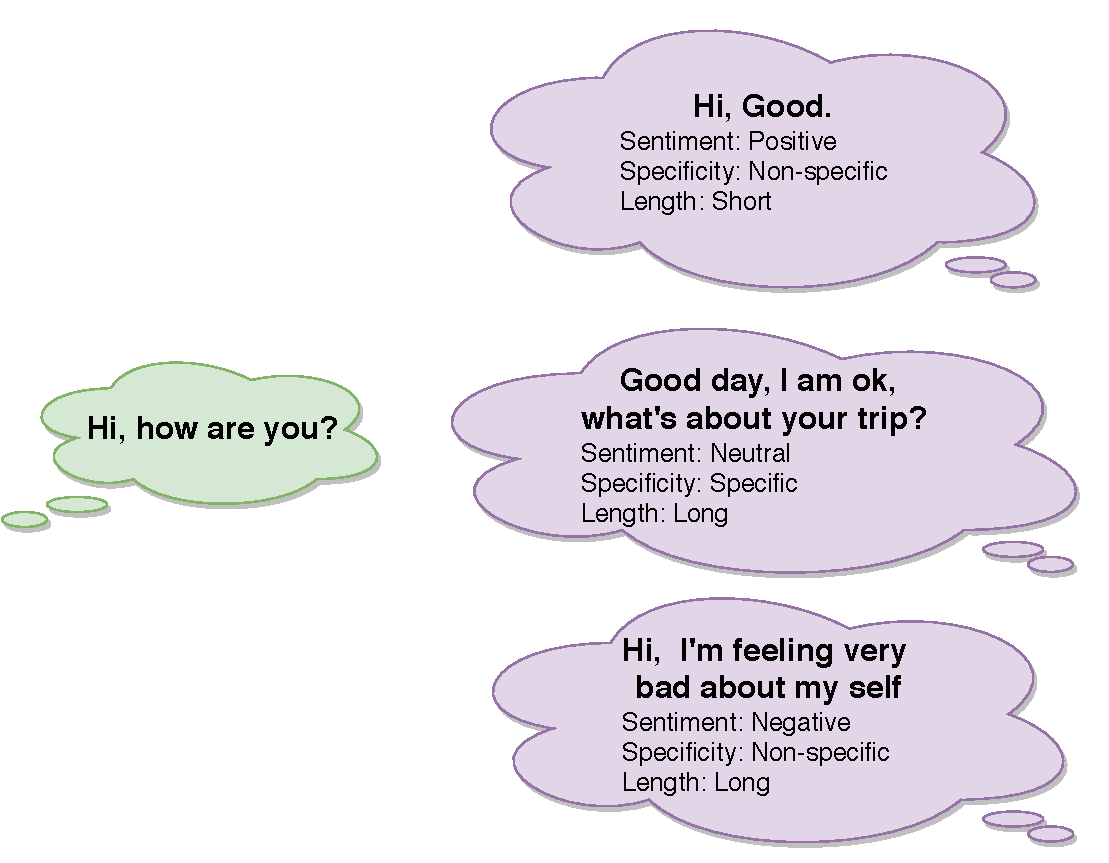
\includegraphics[width=0.6\textwidth]{figures/dialogue_example.pdf}
  \caption{Example of answers to the input sequence with specified attributes.}
  \label{dialogue_example}
\end{figure}

Creating a non-task-oriented DS is a challenge for researchers, because there are a lot of topics of conversations as well as user reactions and responses to them. Such bots often suffer from the inability to generate human-like conversations. Their replies are often too generic, because non-specific responses are in natural language (e.g. ``Ok, I see'', ``I don't know''). 

According to \cite{salovey1990emotional} one of the most important cognitive behaviors in humans is expressing and understanding emotions. That is why it is necessary to pay attention not only to generation of a semantically and syntactically correct text, but also to the emotions and language style in which person communicates to make a dialogue more diverse and interesting. Carefully formulated speech without cliches or jargon is essential to avoid inaccurate presentation and ensure effective communication. Most of the modern generative models are trained on huge corpora which include different contributions from various authors. Texts produced with such models are often not perceived as natural and characterized as non-human, because humans have recognizable writing and communication styles.

The main purpose of this thesis was to create a dialogue system, which is able to generate text in different styles and control the manifestation of each style. Chapter \ref{ds_problems} presents dialogue systems and NLG problems that arise during a dialogue. Chapter \ref{nlg_models} contains the overview of concepts used in the Natural Language Generation. It starts off with an explanation of fundamental techniques common to a lot of machine learning approaches and then continues to describe models specific for NLG and used in the experiments in this thesis. Chapter \ref{related_work} contains a portfolio of current methods and models for solving the problems described in the chapter \ref{ds_problems}. Chapter \ref{eval_datasets_section} describes evaluation methods for NLG in dialogue systems and  publicly available datasets, which are used for the models training in the thesis. Chapter \ref{solution_design} presents designed solution for stylized natural language generation and its evaluation. Implementation of the proposed model architecture is represented in the chapter \ref{chap_implementation}. Chapter \ref{results_discuss} contains the results of the experiments, their analysis and evaluation of the designed model. Chapter \ref{conclusion} summarizes the results reported in the previous chapter and providing recommendations on future research in stylized natural language generation in dialogue systems, which are based on the thesis' results. 

\chapter{Dialogue systems}\label{ds_problems}
NLG is an important component of a DS. According to \cite{alder2017handbook} Natural Language Generation is defined as ``the process by which thought is rendered into language``. NLG approaches can be grouped into two categories, one focuses on generating text using templates or (linguistic) rules (i.e. data-to-text generation), the other uses corpus-based statistical methods (i.e. text-to-text generation), where corpus is a collection of texts \cite{oh2002stochastic}. Spectrum of these approaches along with its (dis)advantages is represented in the Figure \ref{nlg_spectum}.


\begin{figure}[hbt]
  \centering
  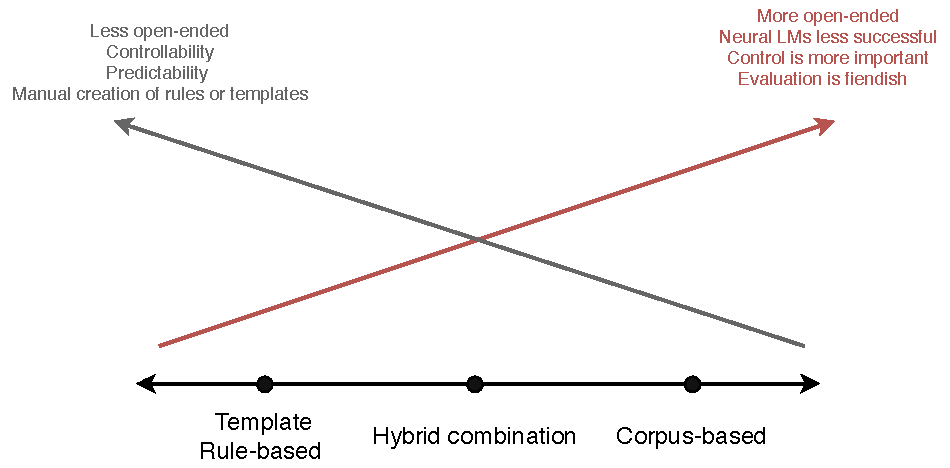
\includegraphics[width=0.9\textwidth]{figures/templateVScorpus.pdf}
  \caption{Spectrum of the NLG approaches.}
  \label{nlg_spectum}
\end{figure}

\section{Template-based approach} 

\begin{table}[ht]
\centering
 \begin{tabular}{|c|} 
 \hline
 Example: \\
 \hline
 User's input: \\
 ``I'm going to travel from Moscow on April 2.'' \\ 
 \hline
 Template: \\
 What time would you like to travel from $\{departure\_city\}$ on $\{departure\_date\}?$ \\
 Repository: $departure\_city$: $\{$Moscow, Brno, Prague$\}$, $departure\_date$: $\{$April 2, March 3$\}$ \\
 \hline
 Agent's output:\\
 ``What time would you like to travel from Moscow on April 2?'' \\
 \hline
 \end{tabular}
 \caption{The example of template-based approach.}
\label{tab:tb_example}
\end{table}

Until recently Natural Language Generation component of a dialog system used primarily hand-coded generation templates, which represented model sentences in a natural language mapped to a particular semantic content.
The template-based system selects a proper response for the current conversation from a repository with response selection algorithms. Templates are often designed for a specific task in a given domain \cite{manishina2016data}. 
Example of template-based system is shown in the Table \ref{tab:tb_example}.


\subsubsection{Advantages of template-based approach}
The pros of template-based approach include that the output produced by this approach is likely to be grammatically correct and not contain unexpected generation errors. The another one is that the process of sentence generation is fully controlled, these models are robust and reliable because they consist of clearly defined rules. 

\subsubsection{Disadvantages of template-based approach}
These models require time and human resources to deploy a real dialogue system, because templates are constructed manually, and the number of templates grows quickly (using different templates for singular and plural versions). The next disadvantage is that human created templates often sound unnatural due to their generic structures. Another weak points are that template-based systems are not able to handle unknown inputs and cannot make variation in output, it is just concatenation of strings. This approach also is not flexible, because it has limits to use templates in other domains. The cons of template-based approach is that a template-based model is not able to learn and is not able to adapt to the user, that's why it generates rigid and stylised responses without the natural variation of human language.

\section{Corpus-based approach}
Corpus-based systems dominate in the NLG community, especially in the case of open-ended tasks, where it is almost impossible to hand-craft the templates for all possible combinations of semantic units. Corpus-based systems include statistical and machine learning approaches to resolve problems of the template-based approach \cite{rudnicky2002dialog}. Corpus-based approach mines large datasets of human-human conversations.

\subsubsection{Advantages of corpus-based approach}
Corpus-based models have ability to generate more proper responses that could have never appeared in the corpus. The next advantage is the ability to mimick the language of a real domain expert and use these models for open-domain dialogue systems. The benefits of corpus-based approach also include that dynamic approach is able to learn and to handle unknown inputs, it is also has a lot of possible variations of output.

\subsubsection{Disadvantages of corpus-based approach}
It is necessary to have a corpus, which contains a large amount of data on a variety of topics to get a sensible output. Even if the corpus is available, process of text generation is not fully controlled and the output can be incorrect or does not need to make a sense. This approach still has a lot of problems, what will be described in more detail in the section \ref{nlg_ds_problems}. 

\section{Language Models}
Corpus-based systems usually rely on \textbf{Language Models(LMs)} to generate sequences of texts. LM is a probabilistic model which estimates the probability of a sequence of words. The Equation \ref{eq:LM} represents the language model, where $W$ is a sequence and $w_1, w_2, ..., w_n$ are words in this sequence. 

\begin{equation} \label{eq:LM}
P(W) = P(w_1, w_2, ..., w_n)
\end{equation}

The \textbf{Chain rule} (Equation \ref{eq:CR}) is commonly employed to factorize the joint probability of a sentence into the product of the conditional probabilities (Equation \ref{eq:CB}) of a word given previous words. 
\begin{equation} \label{eq:CR}
P(w_1, w_2,..., w_n) = \prod_{i}P(w_i|w_1, w_2,...,w_{i-1})
\end{equation}

\begin{equation} \label{eq:CB}
P(A|B) = P(A \cap B) / P(B)
\end{equation}
In Equation \ref{eq:CB} $P(A \cap B)$ is the probability that both events A and B occur.

\begin{figure}[hbt]
  \centering
  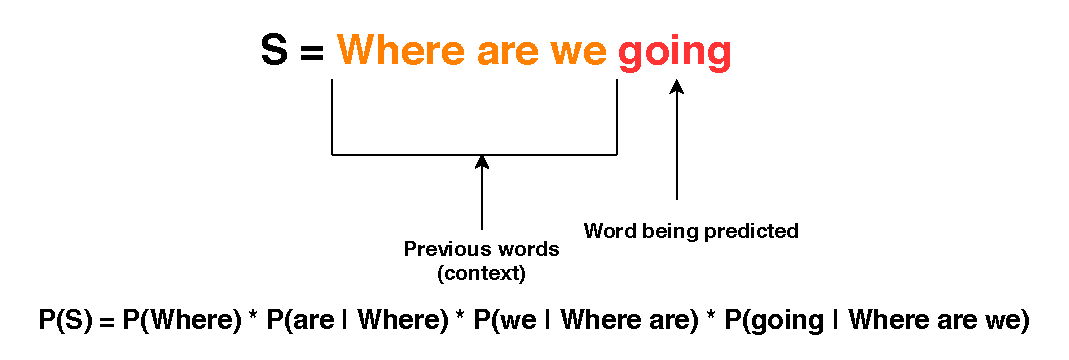
\includegraphics[width=0.8\textwidth]{figures/lm.pdf}
  \caption{Example of calculating a sentence probability by using chain rule.}
  \label{chain_rule}
\end{figure}

An example in the Figure \ref{chain_rule} shows how to predict probability of a word given previous words. A subsequence (context) may consist of a very large number of words and the likelihood that such subsequence is found in a corpus is very small. It is a main problem in language models, which is called \textbf{data sparsity}.

Data sparsity is the phenomenon of not observing enough data in a corpus to model language accurately. The solution to resolve this issue is to make the assumption that the probability of a word depends only on the previous \textit{n} words and use \textbf{N-gram model} (N-gram is a sequence of N words).

\begin{table}[ht]
  \centering
   \begin{tabular}{|c|c|} 
   \hline
    Hi & 1-gram \\
   \hline
    New York & 2-gram \\
   \hline
   The Three Musketeers & 3-gram \\
   \hline
   She is studying IT & 4-gram \\
   \hline
   \end{tabular}
   \caption{The example of N-grams.}
  \label{tab:n_gram}
\end{table}

The n-gram ``She is studying IT'' from the Table \ref{tab:n_gram} does not occur as often in texts of corpus as n-grams ``Hi'', ``New York'' and ``The Three Musketeers''. Knowing a probability to the occurrence of an N-gram in a sequence of words can be useful, because it can help to decide which N-grams can be chunked together to from single entities (like ``New York'' chuncked together as one word). It can also help make next word predictions. For example, ``tea'' is more likely than ``ball'' in the phrase ``I would like to drink''.


According to \cite{bengio2003neural} the state-of-the-art way to fight with data sparsity is learning a distributed representation for words, which allows each training sentence to inform the model about an exponential number of semantically neighboring sentences. The model learns simultaneously a distributed representation for each word along with the probability function for word sequences. A sequence of words that has never been seen before gets high probability if words in this sequence are similar in the sense of having a nearby representation to words forming an already seen sentence. Authors of \cite{bengio2003neural} used neural networks (artificial neural networks are described in the section \ref{nn_section}) for the probability function. The proposed approach improved n-gram models and took an advantage of longer contexts.


\section{Flaws of dialogue systems}\label{nlg_ds_problems}
The ability to communicate with machines in a natural language is a long-standing dream of a mankind. Today's dialogue systems often encounter criticism. There are many scientific works on creating more natural dialogue systems. Markus M. Berg defines a natural dialogue system in \cite{berg2014modelling} as ``a form of dialogue system that tries to improve usability and user satisfaction by imitating human behaviour''. It affects the features of human-to-human dialogue (for example, topic changes, sub-dialogues) and seeks to integrate them into dialogue systems for human interaction with the machine. Open-ended natural dialogue systems still have flaws in generating a response to the user.

\begin{table}[ht]
\centering
 \begin{tabular}{|p{0.5cm}|p{8cm}|p{4cm}|} 
 \hline
 \textbf{\#} & \textbf{Example} & \textbf{Problem type} \\
 \hline
 1 & While Bob ate an apple when it swims. & adequacy\\
 \hline
 2 & Why a mouse when it spins? & adequacy \\
 \hline
 3 & -Yes, I'm studying law at the moment. & repetition\\
   & -Good. & \\
   & -I like playing the piano. & \\
   & -Good.  & \\
\hline
4 & -Do you go get coffee often? & response-relatedness \\
  & -I am a musician. & \\
\hline
5 & -What is your favorite film? & specificity \\
  & -I do not know & \\
  & -What is your hobby? & \\
  & -I have no idea & \\
\hline
 \end{tabular}
 \caption{Examples of DS problems.}
\label{tab:ds_probs}
\end{table}
Main problems of dialogue systems are represented in the Table \ref{tab:ds_probs}. A problem of adequacy shows that a response can be grammatically and syntactically composed correctly, but this sentence does not make sense. A problem of repetition makes conversation boring. A problem of response-relatedness shows that the answer to the question does not make a sense in this context and it spoils the impression of the conversation. A general and trivial response (``I don't know``) in a dialogue could correspond to a very large variety of input sequences, but this does not make the conversation informative and specific.

As noticed in \cite{stent2005evaluating}, the main task of NLG is to select, inflect and order words ``to communicate the input meaning'' as completely, clearly and fluently as possible in context. That's why it is necessary to control if output is appropriate or felicitous in a given context. A good generator usually relies on several factors:
\begin{itemize}
  \item \textbf{adequacy} (a sentence that is ambiguous or not contains communicates meaning in the input, is \textbf{not} adequate)
  \item \textbf{repetition} (self-repetition across sequences and with sequences, repeating the conversational partner)
  \item \textbf{response-relatedness} (efficacy in context)
  \item \textbf{specificity} (informativeness in a dialogue)
  \item \textbf{variation} (there are 2 basic forms of variation: \textit{word choice variation} and \textit{word order variation} for enriching speech)
\end{itemize}

\begin{table}[ht]
\centering
 \begin{tabular}{|p{0.5cm}|p{8cm}|} 
 \hline
 \textbf{\#} & \textbf{Example} \\
 \hline
 1 & I bought movie tickets on Tuesday. \\ 
 \hline
 2 & I got movie tickets on Tuesday. \\
 \hline
 3 & On Tuesday I bought movie tickets. \\
 \hline
 4 & On movie Tuesday tickets I bought. \\
 \hline
 5 & I bought tickets for the Tuesday movie. \\ 
 \hline
 \end{tabular}
 \caption{The example of sentences' variation.}
\label{tab:var_example}
\end{table}

An example in the Table \ref{tab:var_example} shows all types of variation. Sometimes this factor can be syntactically incorrect or unclear, what you can see in the forth sentence. In fifth sentence a variation changed the meaning of part of the sentence. In addition, the variation may add or remove meaning possibilities.


One of the hardest problem in text generation is a language style, which makes a response to an user more human. This task is challenging due to the difficulty of capturing emotional factors and the complex mechanism of human emotions. Some people use obscene speech, some use a lot of expressive means, jargon or jokes to make speech more emotional. This is what distinguishes people and makes their communication more interesting.

\chapter{Concepts in Natural Language Generation} \label{nlg_models}
Development of NLG from static template-like generation to dynamic generation of sentences took a lot of time and models developed along with it. Corpus-based generation uses a generative probabilistic model what can be implemented in many ways. The model focuses on response generation in the context of dialogue, where the task is to generate a response, given an input sequence. Thus, these models fit well within the sequence-to-sequence (seq2seq) (i.e. encoder-decoder) models, which are described in more detail in section \ref{seq2seq_section}. Neural networks are explained for a better understanding seq2seq model.

\section{Neural Networks} \label{nn_section}
Artificial Neural Networks are inspired by biological neural networks. Artificial neuron (Figure \ref{neuron}) is a computational unit in an artificial neural network with a set of real-valued inputs $x_1, x_2 ... x_n$ and an output $y$, where each input $x_i$ has a corresponding weight $w_i$. Weights determine the influence of the input on the output. The neuron's output is the weighted sum of its inputs, which are passed through a non-linear function known as an activation function or transfer function. The transfer functions usually have a sigmoid shape and model the threshold for neuron firing. Bias is an additional parameter in the neural network, which is used to adjust the output along with the weighted sum of the inputs to the neuron. Bias value allows to shift the activation function.

\begin{figure}[hbt]
  \centering
  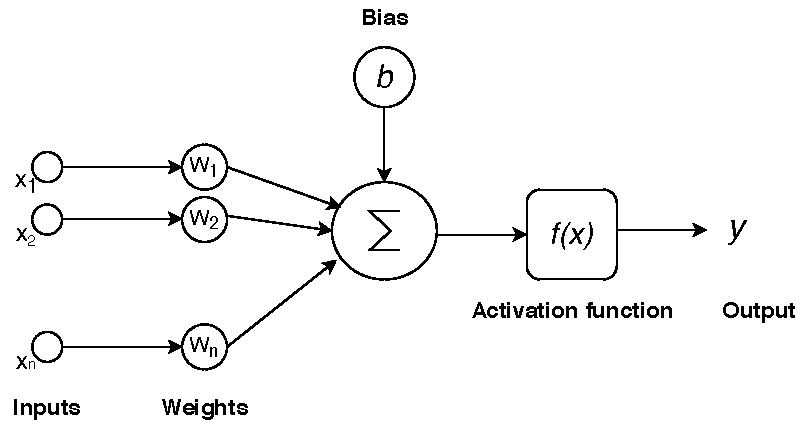
\includegraphics[width=0.5\textwidth]{figures/ai_neuron.pdf}
  \caption{Architecture of an artificial neuron.}
  \label{neuron}
\end{figure}

\begin{figure}[hbt]
  \centering
  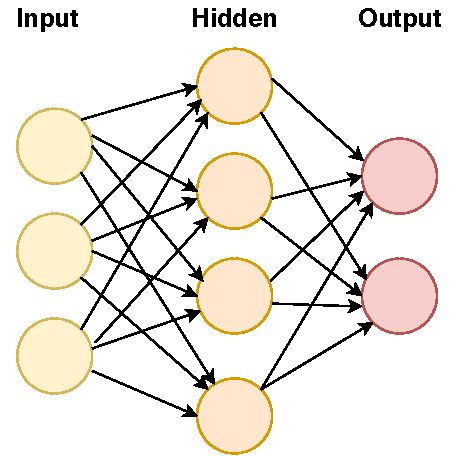
\includegraphics[width=0.3\textwidth, height=0.2\textheight]{figures/nn.pdf}
  \caption{The fully-connected neural network with 1 hidden layer.}
  \label{nn}
\end{figure}

Neurons' outputs can be connected to inputs of other neurons and the calculation is propagated through the network. In fully connected NNs neurons are organized into layers where generally the output of the layer is the input for a next layer. The Figure \ref{nn} represents the most common type of layer -- the fully-connected layer where all neurons between adjacent layers are connected with each other.

The goal of neural network training is to minimize an error (i.e. loss) between predicted outputs of NN and the real data with help of \textbf{Gradient Descent} algorithm \cite{lemarechal2012cauchy}. Gradient Descent finds a local minimum of a differentiable function. \textbf{Backpropagation} \cite{rumelhart1986learning} is used for computing a gradient descent with respect to the weights of NN and for fine-tuning weights. Tuning of the weights ensures lower error rates, what makes a model to approach the true distribution of the data. 

\section{Elman Networks} \label{rnn_section}
Elman Networks are a simple form of recurrent neural networks (RNN) used in natural language processing (NLP) as they allow modelling temporal depedencies of variable length in the data (like context) to be captured. RNNs share the same structure as NNs described in the section \ref{nn_section}, except each layer also has an internal state (i.e. hidden state), which captures information about the previous layer inputs. This allows the network to keep track of past data while processing current inputs.

\begin{figure}[hbt]
  \centering
  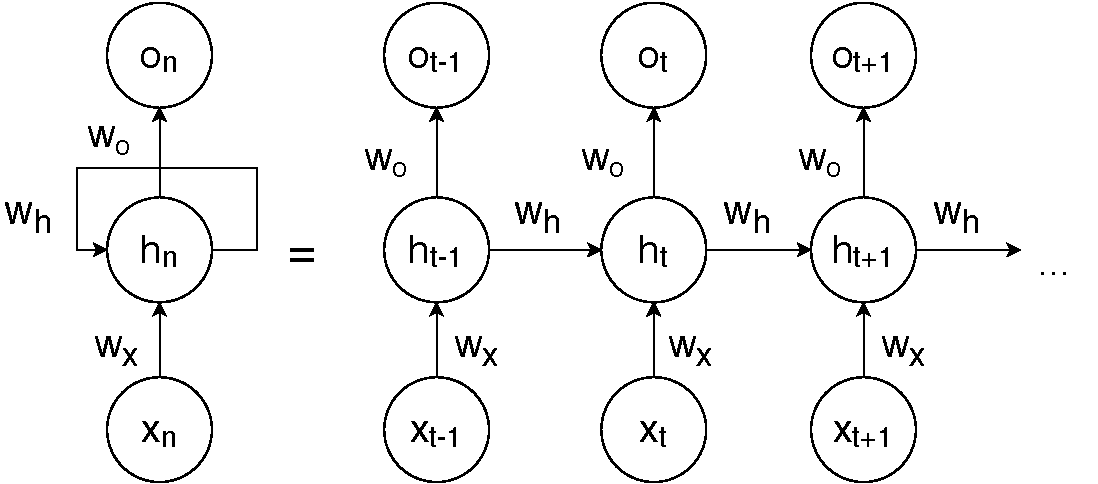
\includegraphics[width=0.5\textwidth]{figures/rnn.pdf}
  \caption{Architecture of Elman neural network, where variable \textbf{h} is a hidden state, \textbf{x} is an input and \textbf{o} is an output. \textbf{w} is a weight, which is optimised to produce a sensible output.}
  \label{rnn}
\end{figure}

The architecture of Elman Networks is illustrated in the Figure \ref{rnn}. A hidden state \textbf{h} is a vector, which calculated from the input $x$ and the previous hidden state. An output \textbf{o} is calculated from this new hidden state. 
The Equations \ref{eq:rnn_h} and \ref{eq:rnn_o} show the formulas for a traditional recurrent neural network.

\begin{equation} \label{eq:rnn_h}
h_t = \sigma(W_hh_{t-1} + W_xx_t)
\end{equation}

\begin{equation} \label{eq:rnn_o}
o_t = softmax(W_oh_t)
\end{equation}

The RNN-based models have been used for NLG as a component of end-to-end trainable task-oriented dialogue system \cite{wen2016network}. 

Nowadays traditional RNN networks almost are not used in NLG, because they have problems with vanishing and exploding gradients. As introduced in \cite{bengio1994learning} these problems occur due to instability of the spectral norm of the Jacobian matrix during training. It happens, because long term components can grow exponentially more then short term ones. The vanishing gradients problem refers to the opposite behaviour. The long term components go exponentially fast to spectral norm 0, which makes it impossible for the model to learn correlation between temporally distant events. This issue has motivated researchers in development of more advanced RNNs like the LSTM \cite{hochreiter1997long}.

\section{Long short-term memory (LSTM)} \label{lstm_section}

\begin{figure}[hbt]
  \centering
  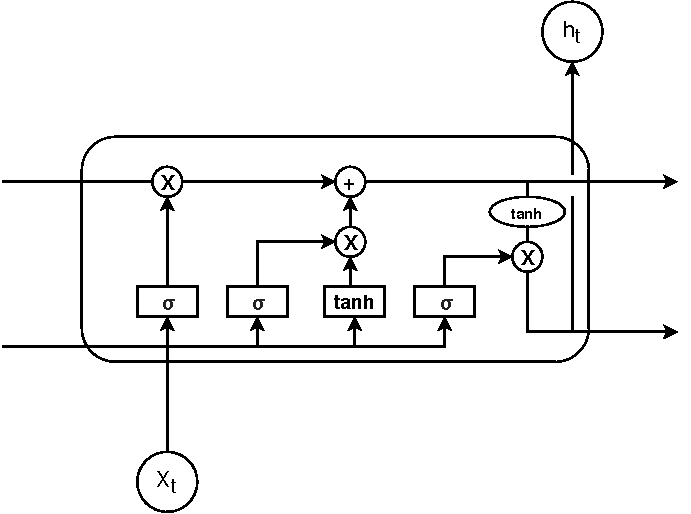
\includegraphics[width=0.5\textwidth]{figures/lstmCell.pdf}
  \caption{A cell in an LSTM network.}
  \label{lstm}
\end{figure}

LSTM networks are a special kind of RNN, which reduce the vanishing gradient problem. It makes them much more effective on capturing long-term dependencies. All recurrent neural networks have the form of a chain of repeating modules of neural network. LSTM network also has this chain structure, but the repeating modules (cells) has a different structure than simple RNN. The key of the solution is usage of multiple gates and a cell state, which runs through all the cells and is manipulated using these gates – parts of the state may be added or removed. Each gate is a sigmoid layer that outputs a number between 0 and 1, which represents the degree of the cell state modification.

The Figure \ref{lstm} represents a structure of a LSTM cell. LSTM cell processes data sequentially for 1 time step and keeps its hidden state through time. First, the network decides how much of information from previous steps to keep stored in its cell state, by using the forget gate, which consists of a sigmoid function applied to weighted sum of previous output, input and bias (Equation \ref{eq:lstm_1}). $W$ are updated through the backpropagation algorithm weights, $b_f$ is a bias, $x_t$ is an input, $h_{t-1}$ is a hidden state from previous step.
\begin{equation} \label{eq:lstm_1}
f_t = \sigma(W_{xf}x_t + W_{hf}h_{t-1}+b_f)
\end{equation}

The next step is to decide how much of the inner state is going to be updated (i.e. what part of the result the cell is going to store in its state), by using input gate (Equation \ref{eq:lstm_2}).
\begin{equation} \label{eq:lstm_2}
i_t = \sigma(W_{xi}x_t + W_{hi}h_{t-1}+b_i)
\end{equation}

After calculating the state modification, it is necessary to compute the new values (i.e. candidate values) which will be stored in it, by using activation function (Equation \ref{eq:lstm_3}).
\begin{equation} \label{eq:lstm_3}
\tilde{c_{t}}=tanh(W_{xc}x_t + W_{hc}h_{t-1} + b_c)
\end{equation}

Updating the cell state is based on the previous state and the candidate values (Equation \ref{eq:lstm_4}). $\odot$ denotes the Hadamard product (element-wise product).
\begin{equation} \label{eq:lstm_4}
c_t = \tilde{c_{t}} \odot i_t + c_{t-1} \odot f_t
\end{equation}

Output gate is represented in Equation \ref{eq:lstm_5}.
\begin{equation} \label{eq:lstm_5}
o_t = \sigma(W_{xo}x_t + W_{ho}h_{t-1}+b_o)
\end{equation}

And the final step producing the hidden state for the next timestep. It is based on the newly updated cell state, transformed by $tanh$ function and multiplied by the output gate (Equation \ref{eq:lstm_6}).
\begin{equation} \label{eq:lstm_6}
h_t = o_t \odot tanh(c_t)
\end{equation}

This model does not suffer so much from a vanishing gradient as simple RNN networks, but still the capacity of the LSTM memory is limited and high computational requirements make learning LSTM difficult. 

\section{Sequence-to-sequence model (seq2seq)} \label{seq2seq_section}

\begin{figure}[hbt]
  \centering
  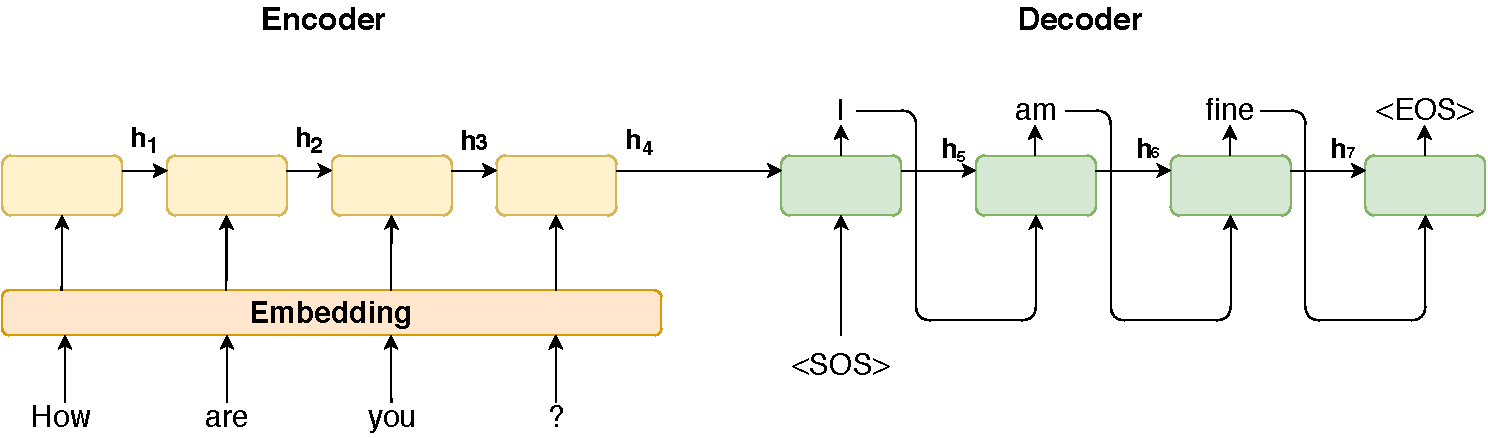
\includegraphics[width=0.8\textwidth]{figures/encoder_decoder.pdf}
  \caption{The architecture of sequence-to-sequence model. $h_i$ represents a hidden state.}
  \label{encoder_decoder}
\end{figure}

Seq2seq models were introduced in 2014 \cite{sutskever2014sequence}. This model uses an encoder-decoder architecture (Figure \ref{encoder_decoder}). Both the encoder and the decoder are recurrent neural networks (vanilla version of RNN is rarely used, because of the problems described in the section \ref{rnn_section}). The role of the encoder is to encode the input, a sequence of variable length data, to a fixed length vector. Decoder based on this vector generates an output sequence of data of different length. These two neural networks are connected into one model to maximise the learning effect. Seq2seq model is very effective in solving NLP problems with long-term dependencies, because input and output sequences can have different lengths and recurrent neural networks can work with ``arbitrarily long'' context. This kind of problems do often appears in machine translation, text summarization, dialogue systems etc.

The Figure \ref{encoder_decoder} presents traditional encoder-decoder arhitecture. Encoder converts an input sequence of words to a corresponding fixed-size hidden vector. Each vector represents the current token and the context of it. 

Every time step, it takes a vector that represents a word and pass its output to the next layer. The last hidden state of encoder passes its output to the first layer of the decoder. The final hidden state of the encoder is also called context vector. The decoder input is an output encoder vector and start token, which characterizes the beginning of the generated sentence. The generated word depends on the previous decoder state and the last generated word.

\section{Decoding strategies} \label{decoding_strategies_section}

Decoding strategies that optimize for output with high probability, such as \textbf{beam search}, make text incoherent and repetitive. A beam search is a limited-width breadth first search. This method starts from an empty sequence $(t=0)$, at every step $t=0, 1, 2, 3,...$ beam search expands at most $k$ partial sequences (with highest probabilities) and computes the probabilities of sequences with length $t+1$. It terminates with a beam of $k$ complete sequences. 

According to \cite{holtzman2019curious} decoding strategies with likelihood maximising lead to text that is degenerate, even when using state-of-the-art models. If the most likely word is always sampled, the model generates repetitive and overly generic text, like ``I don't know'', because it is a typical answer to any question.

Popular sampling methods for generation texts are based on sampling from the distribution. Temperature and top k sampling are the most popular methods to combat sampling from the tail.

\textbf{Temperature sampling} is inspired by statistical thermodynamics, where high temperature means low energy states are more likely encountered. In a probability model logits are divided by the temperature, before feeding them into softmax (Equation \ref{eq:temperature_sampling}, where $t$ is a temperature, $u_{1:|V|}$ are logits). Setting $t \in [0,1)$ skews the distribution towards high probability events, which implicitly lowers the mass in the tail distribution. The temperature parameter controls the shape of distribution without sufficiently suppressing the unreliable tail.

\begin{equation} \label{eq:temperature_sampling}
p(x=V_l|x_{1:i-1}) = \frac{exp(u_l / t)}{\sum_{l'} exp(u_l' / t)}
\end{equation}

\textbf{Top-k sampling} means sorting by probability and probabilities for anything below the token $k$ are set to 0. But in some cases, there are few words to choose, there is a risk of generating bland or generic text, while if $k$ is large the top-k vocabulary will include inappropriate candidates which will have their probability of being sampled increased by the renormalization. The top-k vocabulary $V^{(k)} \subset V$ (the set of size $k$) maximizes $p' = \sum_{x \in V^{(k)}} P(x|x_{1:i-1})$. The distribution is then re-scaled as in Equation \ref{eq:top_K_sampling}.

\begin{equation} \label{eq:top_K_sampling}
P'(x|x_{1:i-1}) = \begin{cases} 
          P(x|x_{1:i-1}) / p' & \mbox{if $x \in V^{(k)}$} \\
          0 & \mbox{otherwise}\\
         \end{cases}
\end{equation}

The research \cite{holtzman2019curious} shows how different natural distribution of human texts and the distribution of machine text produced from maximum likelihood decoding. To resolve this problem authors introduced \textbf{Nucleus Sampling}. The concept is that the vast majority of probabilities are concentrated in a small subset (\textit{nucleus}) of the vocabulary that tends to vary from one to a few hundred candidates. Sampling from the top-$p$ portion of the probability mass expands and contracts the candidate pool dynamically. Formally, given a distribution $P(x|x_{1:i-1})$, the top-p vocabulary $V^{(p)} \in V$ is defined to satisfy the condition in the Equation \ref{eq:nucleus_sampling}, where p is a pre-chosen threshold.

\begin{equation} \label{eq:nucleus_sampling}
\sum_{x \in V^{(p)}} P(x|x_{1:i-1})  \geqslant p
\end{equation}

\section{Attention} \label{attention_section}
A neural attention mechanism is inspired with the human visual attention mechanism. Visual attention is able to focus on a certain region of an image with ``high resolution'', while perceiving the surrounding image in “low resolution”, and then adjusting the focal point over time. An example of the attention mechanism is represented in the Figure \ref{fig:attention}.

\begin{figure}[hbt]
  \centering
  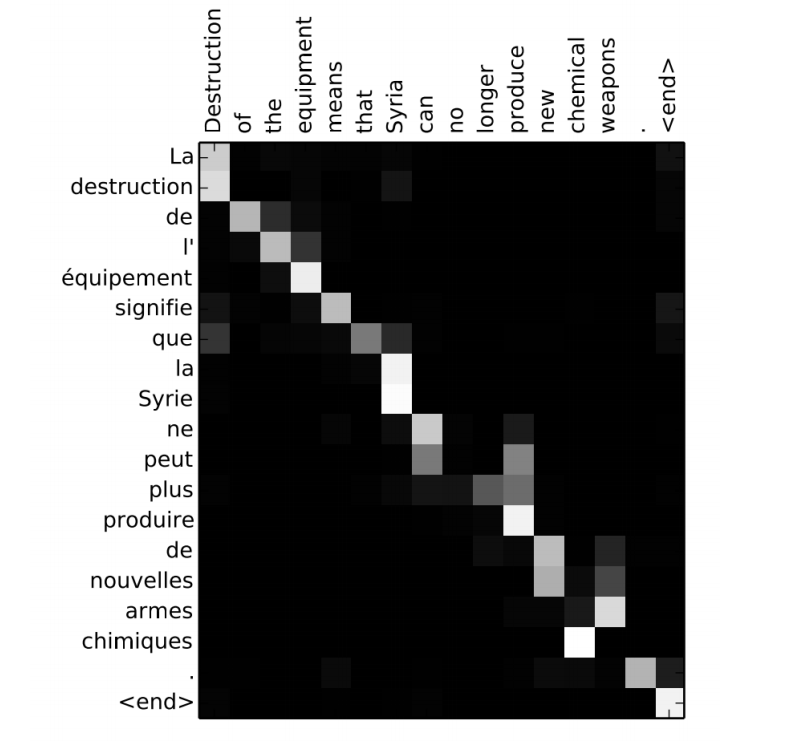
\includegraphics[width=0.5\textwidth]{figures/attention_example.png}
  \caption{An example of attention mechanism. The x-axis and y-axis correspond to the words in the input sequence in English and the generated translation in French. Each pixel represents a weight.\protect\footnotemark}
  \label{fig:attention}
\end{figure}

\footnotetext{\url{https://arxiv.org/pdf/1409.0473.pdf}}

\begin{equation} \label{eq:attention}
output_i = \sum_{j=1}^{T} \alpha_{ij} h_j
\end{equation}
 
In the Equation \ref{eq:attention} an output of the attention mechanism for time $i$ is represented. $T$ is a length of an input sequence, $h_j$ is a hidden state representing a value, $\alpha_{ij}$ (Equation \ref{eq:attention_w}) is a weight of each annotation $h_j$.

\begin{equation} \label{eq:attention_w}
\alpha_{ij} = \frac{exp(e_{ij})}{\sum_{k=1}^{T} exp(e_{ik})}
\end{equation}

\begin{equation} \label{eq:alignment_model}
e_{ij} = a(s_{i-1}, h_j)
\end{equation}

In the Equation \ref{eq:alignment_model} $e_{ij}$ represents an alignment model, represented as feedforward neural network $a$, which scores how well match the inputs around position $j$ and the output at position $i$. $s_{i-1}$ is RNN hidden state.

In \cite{vaswani2017attention} attention is described as ``mapping a query and a set of key-value pairs to an output, where the query, keys, values, and output are all vectors''. The output represents a computed weighted sum of the values (Equation \ref{eq:attention}). A weight for each value is computed by a compatibility function of the query with the corresponding key. Weights for keys corresponding to important values will be greater than for unimportant ones, which means that important values will be a bigger part of the output. 

Self-attention is an attention mechanism, where ``self`` means that the inputs interact with each other and ``attention`` means that inputs find out who they should pay more attention. In the self-attention mechanism the query, keys and values are from the same sequence. The query is a single element from the sequence while the keys and values are the entire sequence. The attention output is a new representation of the element that was the query. Self-attention is used to compute a new representation of the sequence.  

\section{Luong attention}\label{sec_luong}

\begin{figure}[hbt]
  \centering
  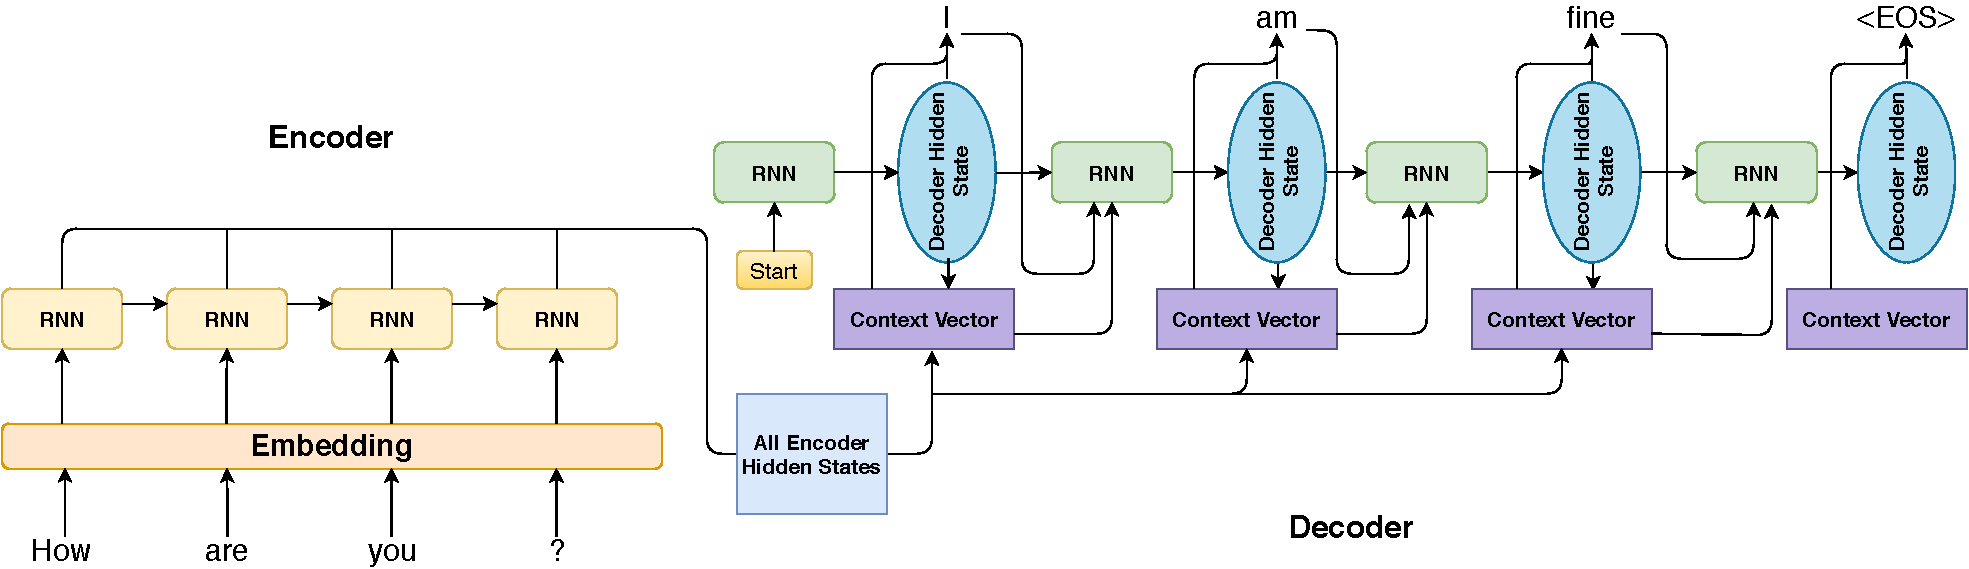
\includegraphics[width=0.9\textwidth]{figures/luong_decoder.pdf}
  \caption{A seq2seq model with Luong attention.}
  \label{fig:luong}
\end{figure}

Luong attention model \cite{luong2015effective} (Figure \ref{fig:luong}) is classified into 2 categories, \textit{global} and \textit{local}. Common to these types of model is the fact that at each time step \textit{t} in the decoding phase previous hidden state is taken as input to derive a context vector $\mathbf{c_t}$, that captures relevant information to predict the current target word $y_t$. This categories differ only if ``attention'' is placed on all source positions or on a few source positions.

The simple concatenation layer combines the information from vectors $h_t$ and $c_t$ to produce an attentional hidden state (Equation \ref{eq:hs}).
\begin{equation} \label{eq:hs}
\mathbf{\widetilde{h_t}} = tanh(\mathbf{W_c}[\mathbf{c_t};\mathbf{h_t}])
\end{equation}

The attentional hidden state $\mathbf{\widetilde{h_t}}$ then passed through the softmax layer to produce the predictive distribution (Equation \ref{eq:sfm}).
\begin{equation} \label{eq:sfm}
p(y_t|y_{<t},x) = softmax(\mathbf{W_s}\mathbf{\widetilde{h_t}})
\end{equation}

\subsubsection{Global Attention}
An alignment vector $a_t$ (size of $a_t$ is equal to the number of time steps on the source side) is derived by comparing the current target hidden state $\mathbf{h_t}$ with each source hidden state $\mathbf{\bar{h}_s}$ (Equation \ref{eq:av}).
\begin{equation} \label{eq:av}
a_t(s) = align(\mathbf{h_t}, \mathbf{\bar{h}_s}) = \frac{exp(score(\mathbf{h_t}, \mathbf{\bar{h}_s}))}{\sum_{s'} exp(score(\mathbf{h_t}, \mathbf{\bar{h}_s}))}
\end{equation}

There are three common types of the score function (the score function is referred as a content-based function) (Equation \ref{eq:sf}).
\begin{equation}\label{eq:sf}
score(\mathbf{h_t}, \mathbf{\bar{h}_s}) = \begin{cases} \mathbf{h_t}^\intercal \mathbf{\bar{h}_s}, & \mbox{dot} \\ \mathbf{h_t}^\intercal \mathbf{W_a} \mathbf{\bar{h}_s}, & \mbox{general} \\ \mathbf{v_a}^\intercal tanh(\mathbf{W_a} [\mathbf{h_t}; \mathbf{\bar{h}_s}]), & \mbox{concat} \end{cases}
\end{equation}

In location-based function the alignment scores are computed from solely the target hidden state $\mathbf{h_t}$ (Equation \ref{eq:sfm_as}).
\begin{equation} \label{eq:sfm_as}
a_t = softmax(\mathbf{W_a}\mathbf{h_t})
\end{equation}

The context vector $\mathbf{c_t}$ is computed as the weighted average over all the source hidden state, where alignment vector represents weights.

\subsubsection{Local Attention}
Global attention is expensive, because it has to attend to all words on the source side for each target word. Local attention chooses to focus only on a small subset of the source positions per target word.

The local alignment vector $a_t$ in this category of attention is fixed-dimensional, because of it there are 2 variants of the model, \textit{monotonic} (Equation \ref{eq:monotonic}) and \textit{predictive} (Equation \ref{eq:predictive}).

\begin{equation} \label{eq:monotonic}
p_t = t
\end{equation}

\begin{equation} \label{eq:predictive}
p_t = S \cdot sigmoid(\mathbf{v_p}^\intercal tanh(\mathbf{W_p} \mathbf{h_t}))
\end{equation}

In monotonic alignment the source and target sequences are roughly monotonically aligned. In predictive alignment the model learns to predict the alignment position, where $\mathbf{W_p}$ and $\mathbf{v_p}$ are the learned model parameters.

Gaussian distribution centered in $p_t$ is used to favor alignment points near $p_t$ (Equation \ref{eq:align_gaus}).
\begin{equation} \label{eq:align_gaus}
a_t(s) = align(\mathbf{h_t}, \mathbf{\bar{h}_s}) exp(-\frac{(s-p_t)^2}{2\sigma^2})
\end{equation}

\section{Transformer} \label{sec_transformer}

The transformer \cite{vaswani2017attention} follows the seq2seq architecture that is based on self-attention mechanism. The model does not use any recurrent networks. In each step this model applies self-attention mechanism which directly models relationships between all words in a sequence, regardless of their respective position. Transformers do not require that the sentence be processed in order, that allows process parallelization during training, unlike RNN. 

\begin{figure}
  \centering
  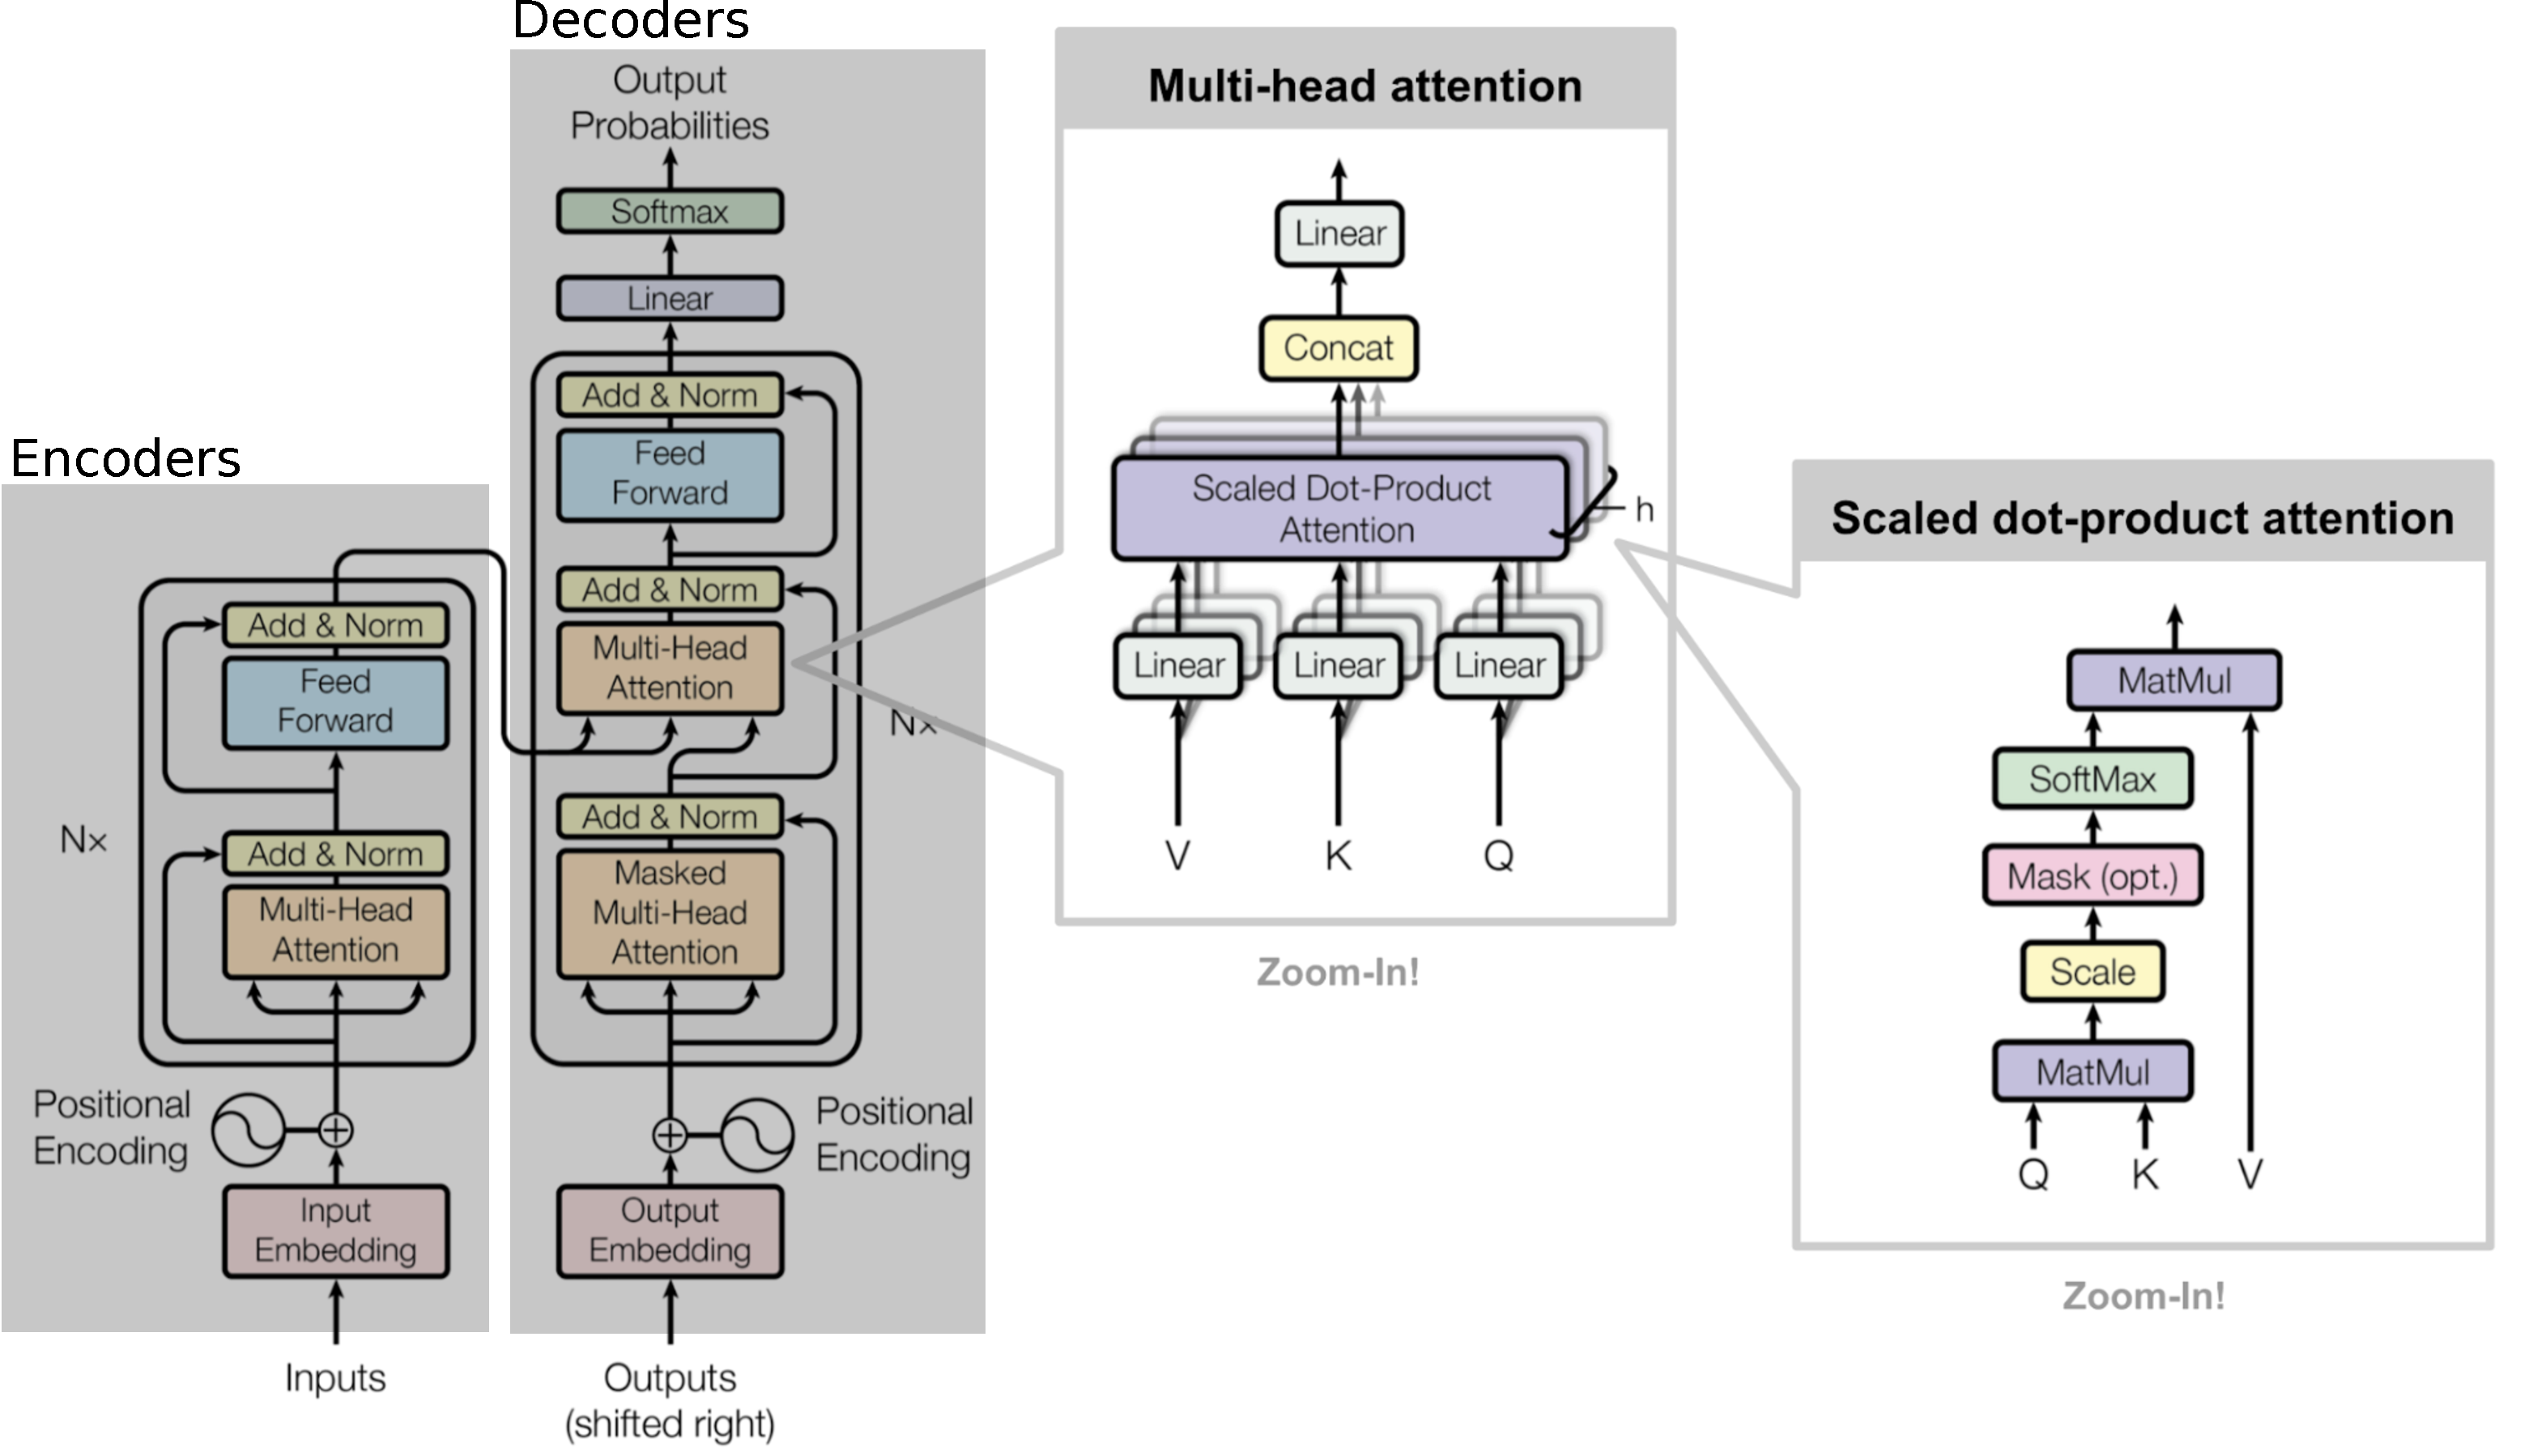
\includegraphics[width=0.9\textwidth]{figures/transformer_attention.pdf}
  \caption[Transformer architecture]{The architecture of the Transformer.\protect\footnotemark}
  \label{fig:transformer}
\end{figure}

\footnotetext{\url{http://primo.ai/index.php?title=Transformer}}

\begin{equation} \label{eq:transformer_attention}
Attention(Q, K, V) = softmax(\frac{QK^T}{\sqrt{d_k}})V
\end{equation}

\begin{equation} \label{eq:transformer_multi_head}
MultiHead(Q, K, V) = Concat(head_1, head_2, ..., head_h)W^O
\end{equation}

An Equation \ref{eq:transformer_attention} represents a \textbf{scaled dot-product attention}. The input consists of values of dimension $d_v$, queries and keys of dimension $d_k$, where queries, keys and values are matricies.

An Equation \ref{eq:transformer_multi_head} represents a \textbf{multi-head attention}, which allows the model to jointly track information from different representation subspaces at different positions. Averaging inhibits this with a single head of attention. The input also consists of queries, keys and values matricies, $W^O$ is a parameter matrix, $h$ is a number of parallel layers, $head_i = Attention(QW_i^Q, KW_i^K, VW_i^V)$, where $W_i^Q, W_i^K, W_i^V$ are parameter matricies. $Q$, $K$ and $V$ are different for each position of the attention modules in the structure. It depends on if they are in the encoder, the decoder or between them.

The architecture of the transformer is illustrated in the Figure \ref{fig:transformer}. $N_x$ in this Figure represents the number of encoder or decoder identical layers that can be stacked on top of each other multiple times. The inputs and output are first embedded into an n-dimensional space. Words' positions, n-dimensional vector, are added to the embedded representation of each word (Equation \ref{eq:pe}). These positions are used to inject some information about the relative or absolute position, because the transformer does not contain recurrence and convolution. 

\begin{eqfloat} [H]
\begin{equation} \label{eq:pe}
\begin{array}{lcl} 
PE_{(pos, 2i)} = sin(\frac{pos}{10000^{\frac{2i}{d_{model}}}}) \\

PE_{(pos, 2i+1)} = cos(\frac{pos}{10000^{\frac{2i}{d_{model}}}})\\
\end{array}
\end{equation}
\caption{The functions for calculating a word's positional encoding, where $pos$ is a position, $i$ is a dimension, $d_{model}$ is the same dimension as the embeddings.}
\end{eqfloat}

The transformer consists of a stack of encoders, where an encoder maps an input to a sequence of continuous representations. Each encoder has two sub-layers, where the first one is a multi-head self-attention mechanism, and the second is a simple, position-wise fully connected feed-forward network. There is a residual connection \cite{he2016deep} around each of the two sub-layers, followed by layer normalization \cite{ba2016layer}. All sub-layers in the model produce outputs of dimension $d_{model}$, as well as the embedding layers.

The transformer also consists of a stack of decoders. In addition to the two sub-layers in each encoder, a decoder has an extra sub-layer, which performs multi-head attention over the output of the encoder stack. Masking in this layer ensures that the predictions for position $k$ can depend only on the known outputs at positions less than $k$. There is also the residual connection. 

\section{Generative Pre-Training (GPT)} \label{sec_gpt}
GPT \cite{radford2018improving} is a transformer-based (Section \ref{sec_transformer}) language model. The model works in 2 stages. First of all transformer model trained on a very large amount of data in an unsupervised manner, then the model is fine-tuned on much smaller supervised dataset to help it solve specific tasks.

\subsubsection{Unsupervised pre-training}
In unsupervised pre-training a standard language modelling is used and the aim is to maximize the likelihood (Equation \ref{eq:unsupervised_pre_training}, where $U = {u_1, u_2, ... , u_n}$ is an unsupervised corpus of tokens, $k$ is the size of context window, $P$ is modeled using a neural network with parameter $\Theta$).

\begin{equation} \label{eq:unsupervised_pre_training}
L_1(U) = \sum_i \log P(u_i|u_{i-k}, ... , u_{i-1}; \Theta)
\end{equation}

Multi-layer transformer decoder is used for the language model. The model applies a multi-headed self-attention operation over the input context tokens followed by position-wise feedforward layers to produce an output distribution
over target tokens (Equation \ref{eq:unsupervised_decoder}), where $U = (u_{-k}, ... , u_{-1})$ is the context vector of tokens, $n$ is the number of layers, $W_e$ is the token embedding matrix, $W_p$ is the position embedding matrix).

\begin{equation}  \label{eq:unsupervised_decoder}
\begin{array}{lcl} 
h_0 & = &UW_e + W_p \\

h_l & = & transformer\_block(h_{l-1}) \forall l \in [1,n] \\

P(u) & = & softmax(h_n W_e^T) \\
\end{array}
\end{equation}

\subsubsection{Supervised fine-tuning}
After training the model, the parameters are adapted to the supervised target task. Given a labeled dataset $C$, where an instance represents a sequence of input tokens $(x^1, ... , x^m)$, along with a label $y$. The inputs are passed through the pre-trained model to get the final transformer block's activation $h_l^m$, which is then fed into an additional linear output layer with $W_y$ parameters for predicting $y$ (Equation \ref{eq:supervised_fine_tune}). 

\begin{equation} \label{eq:supervised_fine_tune}
P(y|x^1, ... , x^m) = softmax(h_l^{m\intercal} W_y)
\end{equation}

\begin{equation} \label{eq:supervised_maximize}
L_2(C) = \sum_{(x,y)} \log P(y|x^1, ... , x^m)
\end{equation}

Authors found that including language modelling as an auxiliary objective to the fine-tuning helped learning. First of all it improves the generalization of the supervised model. Secondly it accelerates convergence. They optimize the objective with weight $\lambda$ (Equation \ref{eq:objective_optimalization}).

\begin{equation} \label{eq:objective_optimalization}
L_3(C) = L_2(C) + \lambda * L_1(C)
\end{equation}

\section{BART} \label{bart_section}

\begin{figure}[hbt]
  \centering
  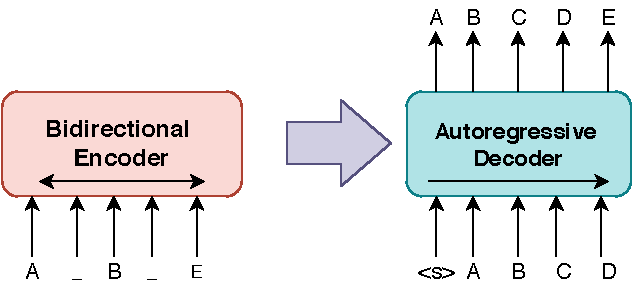
\includegraphics[width=0.5\textwidth]{figures/BART.pdf}
  \caption{BART: Encoder inputs need not be aligned with decoder outputs, it allows arbitary noise transformations. A document is corrupted by replacing spans of text with mask symbols. The corrupted document is encoded with a bidirectional model, and then the likelihood of the original document is calculated with an autoregressive decoder. For fine-tuning, an uncorrupted document is input to both the encoder and decoder, and representations from the final hidden state of the decoder are used \cite{lewis2019bart}.}
  \label{fig:bart}
\end{figure}

BART (Figure \ref{fig:bart}) is a denoising autoencoder for pre-training sequence-to-sequence models that maps a corrupted document to the original document it was derived from. The model uses a standard transformer-based seq2seq architecture, with a bidirectional encoder and left-to-right decoder.

Bidirectional encoder consists of $N$ transformer encoder blocks stacked on top of each other (Section \ref{sec_transformer}), output is taken from the final block. The input is a sequence of tokens, which are first embedded into vectors and the processed in the model. The output is a sequence of vectors of size $H$, in which each vector corresponds to an input token with the same index. Autoregressive decoder is GPT model (Section \ref{sec_gpt}). Authors modified ReLU activation functions (Equation \ref{eq:relu}) to GELU (Equation \ref{eq:gelu}) and initialized parameters from $\mathcal{N}(0, 0.2)$. Autoregressive decoder can be directly fine tuned for sequence generation tasks.

\begin{eqfloat} [H]
\begin{equation} \label{eq:relu}
f(x) = x^+ = max(0, x)
\end{equation}
\caption{Rectified Linear Unit (ReLU).}
\end{eqfloat}
\begin{eqfloat} [H]
\begin{equation} \label{eq:gelu}
GELU(x) = xP(X \leq x) = x \Phi(x)
\end{equation}
\caption{Gaussian Error Linear Unit (GELU), where $P$ is a Gaussian Probability Density Function.}
\end{eqfloat}

Pre-training has two stages: text corruption with an arbitrary noising function and learning to reconstruct the original text. BART allows to apply any type of document corruption, such as token masking, sentence permutation, document rotation, token deletion, text infilling (Figure \ref{fig:bart_doc_corruption}).

\begin{figure}[hbt]
  \centering
  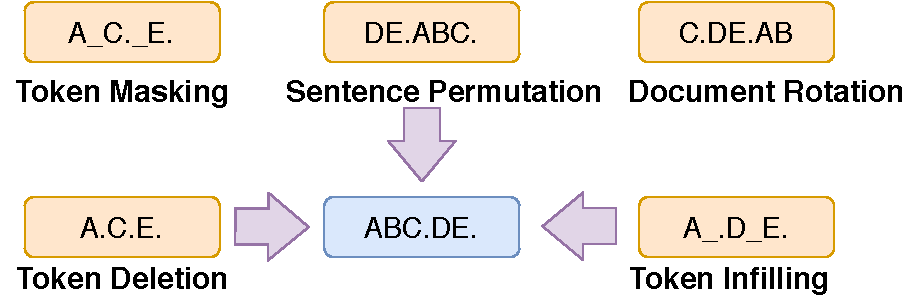
\includegraphics[width=0.6\textwidth]{figures/bart_doc_corruptions.pdf}
  \caption{Corruptions for noising the input. These transformations can be composed.}
  \label{fig:bart_doc_corruption}
\end{figure}

In \textbf{Token Masking} part of words in each sequence are replaced with a \texttt{[MASK]} token before embedding. The model then tries to predict the original value of the masked words, based on the context provided non-masked words in the sequence. Bidirectional encoder loss function takes into consideration only the prediction of masked values. Pre-training on this task allows the model to learn general features of the language.

In \textbf{Token Deletion} random tokens are deleted from the input. It is needed to decide which positions are missing inputs.

For \textbf{Text Infilling} a number of text spans are sampled. Span lengths represent a Poisson distribution ($\lambda=3$) and each span is replaced with a single \texttt{[MASK]} token. The model learns to predict how many tokens are missing from a span.

In \textbf{Document Rotation} a token is chosen uniformly at random. A document rotation starts with that token. The model learns to identify the start of the document.

For \textbf{Sentence Permutation} a document is divided into sentences based on full stops (full stop is a punctuation marking the end of a declarative sentence). These sentences are randomly shuffled.

\chapter{Related work} \label{related_work}
This chapter presents an overview of the most popular NLG models for building open-ended dialogue systems. 

Modelling conversations with generative probabilistic models was first proposed in \cite{ritter2011data}. They present a data-driven approach to generating responses to Twitter status posts, based on phrase-based Statistical Machine Translation. In \cite{shang2015neural} authors proposed a framework for generating responses on micro-blogging websites with using recurrent neural networks. Their model can generate grammatically correct and content-wise appropriate responses to over 75\% of the input text. 

The idea that computers can generate stylized texts already appeared half a century ago in \cite{wheatley1965computer}. Authors choose a variety of text characteristics as style, such as an expession of politeness in machine translation \cite{sennrich2016controlling}, transformation from modern English to Shakespearean English \cite{jhamtani2017shakespearizing}, sentiment of a text in \cite{shen2017style} and \cite{li2018delete}. In \cite{gao2019structuring} authors used a structured latent space to generate stylized dialogue responses. Another approach was proposed in \cite{john2018disentangled}, where authors applied an adversarial loss to separate style from content. In \cite{tikhonov2018guess} authors describe the problem of stylized text generation in a multilingual setup and show the importance of phonetics for generating the author's stylized poetry.

\section{Attributes control}

In \cite{see2019makes} solutions to common NLG problems in dialogue systems are described. Authors add control (the ability to specify desired attributes of the generated text at test time) and focus on four controllable attributes of text: repetition, specificity, response-relatedness and question-asking. They measure repetitiveness as n-gram overlap, specificity as word rareness, response-relatedness as the embedding similarity of the bot’s response to the human’s last sequence. In this work, authors use \textbf{Conditional Training (CT)} \cite{peng2018towards} and \textbf{Weighted Decoding (WD)} \cite{ghazvininejad2017hafez}. 

\begin{figure}[hbt]
  \centering
  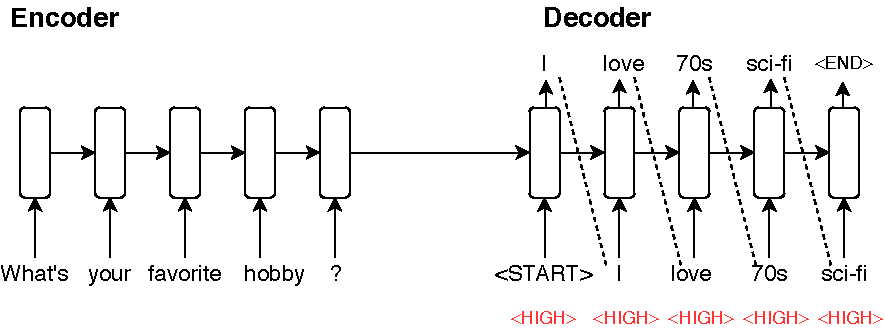
\includegraphics[width=0.7\textwidth]{figures/ct.pdf}
  \caption{Example of Condition Training model.}
  \label{fig:ct}
\end{figure}

A \textbf{CT} model learns probabilities $P(y|x,z)$, where $y$ is the output text, $x$ is the input text and $z$ is a control variable, which specifies the desired output attribute. In the model $z$ is presented with learned embedding and is concatenated to each decoder input. For example, to get very generic or very specific response, $z$ can be set to an embedding representing \texttt{<LOW>} or \texttt{<HIGH>} (Figure \ref{fig:ct}). If it is necessary simultaneously control several attributes, multiple control embeddings ($z_1, z_2, ..., z_n$) can be concatenated and the model learns $P(y|x, z_1, z_2, ..., z_n)$. Disadvantage of Conditional Training is that it can’t control attributes without sufficient training data. Another observed flaw is that the CT model learns only a very weak connection between $z$ and the semantic relatedness of the output.

A \textbf{WD} is a technique applied during decoding to increase/decrease the probability of words with certain features. 
\begin{equation} \label{eq:wd}
score(w, y_{<t}; x) = score(y_{<t}; x) + \log P_{RNN}(w|y_{<t}, x) + \sum_i w_i * f_i(w; y_{<t}, x)
\end{equation}
In weighted decoding (Equation \ref{eq:wd}), a hypothesis $y_{<t} = y_1, ..., y_{t-1}$ is expanded by computing the score for each possible next word $w$ in the vocabulary on the $t^{th}$ step of decoding. $\log P_{RNN}(w|y_{<t}, x)$ is the log-probability of the word $w$ assigned by the probabilistic model. $score(y_{<t}; x)$ is the accumulated score of the already-generated words in the hypothesis $y_{<t}$. $f_i(w; y_{<t}, x)$ is a decoding feature with associated weights $w_i$ (hyperparameters to be chosen). Each feature presents a specific controlling attribute.

\begin{equation} \label{eq:nidf}
NIDF(w) = \frac{IDF(w) - min\_idf}{max\_idf - min\_idf}
\end{equation}
\textbf{Normalized Inverse Document Frequency (NIDF)} is used as a measure of word rareness. In conditional training the metric is represented as $z$ variable and in weighted decoding as a parameter of rareness for a word prediction (On each step of the decoding, the probability of each word in the vocabulary is updated in proportion to its rareness. The size of the update is controlled by a weight parameter.) (Equation \ref{eq:nidf}). $IDF(w) = \log(\frac{R}{c_w})$ is a Inverse Document Frequency of a word $w$, where $R$ is the number of responses in the dataset, $c_w$ is the number of those responses that contain $w$. $min\_idf$ and $max\_idf$ are the minimum and maximum IDF's, which are used for normalising the NIDF (ranges from 0 to 1).

\section{Emotional Chatting Machine (ECM)}
Emotional Chatting Machine (ECM) \cite{zhou2018emotional} can generate not only relevant and grammatical responses, but also emotionally consistent. This framework proposes seq2seq architecture. This separate responses into several categories (Angry, Disgust, Happy, Like, Sad, Other). The emotion category of the to-be-generated response is given for ECM, because, according to the authors, emotions are highly subjective. 

\begin{figure}[hbt]
  \centering
  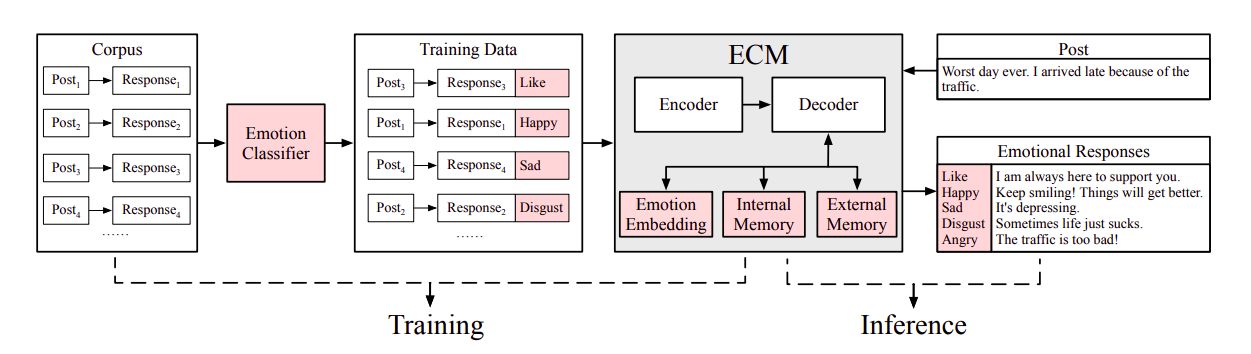
\includegraphics[width=1\textwidth]{figures/ecm.png}
  \caption{Overview of ECM (the grey unit). The pink units are used to model emotion factors in the framework.}
  \label{fig:ecm}
\end{figure}

In the architecture (Figure \ref{fig:ecm}) a post can be answered with different emotions, depending on the attitude of the respondent. For example, for a sad story, someone may respond with anger  (as an irritable stranger), sympathy (as a friend) or happy (as an enemy). \textit{Emotion classifier} generates labels for each response. Generated labels and responses are fed into ECM to generate emotional responses conditioned on different emotion categories. 

\begin{eqfloat}
\begin{equation} \label{eq:emotion_cat_emb}
s_t = GRU(s_{t-1},[c_t; e(y_{t-1}); v_e])
\end{equation}
\caption{ECM decoder's state. GRU \cite{cho2014learning} is a gating mechanism in RNN.}
\end{eqfloat}

In \textit{Emotion Category Embedding} (Equation \ref{eq:emotion_cat_emb}) each emotion category of a response is represented by a real-valued, low dimensional vector. The vector of an emotion category $v_e$ for each category $e$ is randomly initialize. During the training the model is learning the vectors of the emotion category. The emotion category embedding, along with the context vector $c_t$, and the word embedding $e(y_{t-1})$, are fed into the decoder to update the decoder's state $s_t$. 

\begin{figure}[H]
  \centering
  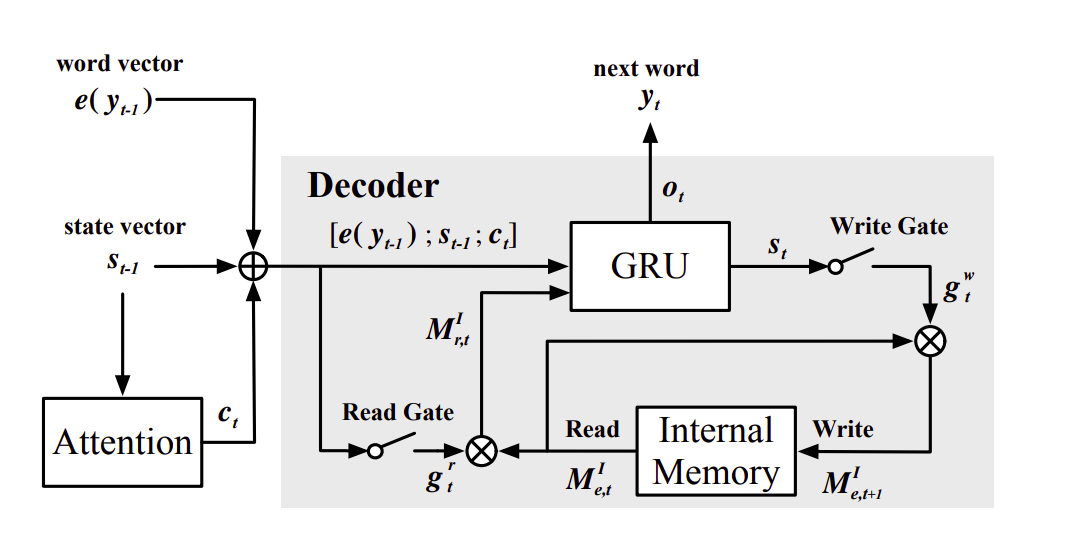
\includegraphics[width=0.5\textwidth]{figures/internal_memory.png}
  \caption{Data flow of the decoder with an internal memory.}
  \label{fig:internal_memory}
\end{figure}

\begin{equation} \label{eq:read_gate}
g_t^r = \sigma(W_g^r[e(y_{t-1}); s_{t-1}; c_t])
\end{equation}

\begin{equation} \label{eq:write_gate}
g_t^w = \sigma(W_g^w s_t)
\end{equation}

\textit{Internal memory} captures emotion dynamics during decoding. It is achieved using the following concept: before the decoding process each category has an internal emotion state; at each step the emotion state decays by a certain amount; when decoding process is completed, the emotion state should be zero, what indicates that the emotion is completely expressed. The detailed process is represented in the Figure \ref{fig:internal_memory}, where at each time step $t$, the gate $g_t^r$ (Equation \ref{eq:read_gate}) is computed with the input of the word embedding of the previously decoded word $e(y_{t-1})$, the previous state vector of the decoder $s_{t-1}$, and the current context vector $c_t$. The write gate $g_t^w$ (Equation \ref{eq:write_gate}) is computed on the decoder's state $s_t$. These gates are used to read from and write into the internal memory.

\begin{equation} \label{eq:im_r}
M_{r,t}^I = g_t^r \odot M_{e,t}^I
\end{equation}

\begin{equation} \label{eq:im_w}
M_{e,t+1}^I = g_t^w \odot M_{e,t}^I
\end{equation}

The emotion state is erased by a $g_t^w$ at each time step. At the last step, the internal emotion state will decay to zero. This process is represented in the Equations \ref{eq:im_r}, \ref{eq:im_w}, where $M$ means memory, $I$ denotes Internal, $r/w$ denotes read and write respectively, $\odot$ is element-wise multiplication.

\begin{equation} \label{eq:im_state}
s_t = GRU(s_{t-1},[c_t; e(y_{t-1}); M_{r,t}^I])
\end{equation}

The decoder's state $s_t$ is conditioned on the previous state of the decoder $s_{t-1}$, the context vector $c_t$, the previous target word $e(y_{t-1})$ and the emotion state update $M_{r,t}^I$ (Equation \ref{eq:im_state}).

\textit{External memory} is used to model emotion expressions explicitly, because in the internal memory module the correlation between the change of the internal emotion state and selection of a word is not directly observable. The model can choose to generate words from  an emotion vocabulary or a generic vocabulary.

\begin{figure}[H]
  \centering
  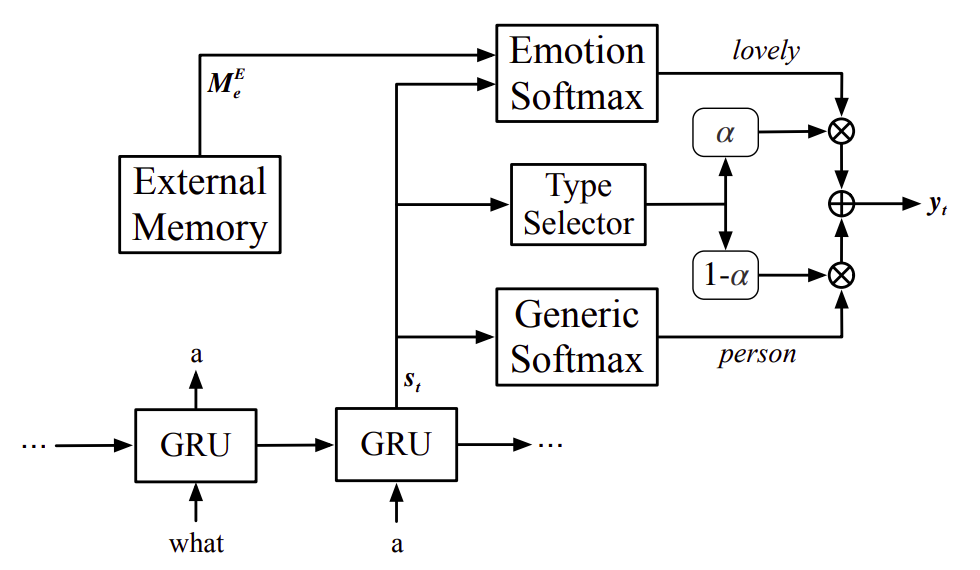
\includegraphics[width=0.5\textwidth]{figures/external_memory.png}
  \caption{Data flow of the decoder with an external memory.}
  \label{fig:external_memory}
\end{figure}

\begin{equation} \label{eq:ex_alpha}
\alpha_t = \sigma(v_u^\intercal s_t)
\end{equation}

\begin{equation} \label{eq:ex_emotion_sfmx}
P_g(y_t = w_g) = softmax(W_g^o s_t)
\end{equation}

\begin{equation} \label{eq:ex_generic_sfmx}
P_e(y_t = w_e) = softmax(W_e^o s_t)
\end{equation}

\begin{equation}\label{eq:ex}
y_t \sim o_t = P(y_t) = \begin{cases} (1-\alpha_t)P_g(y_t = w_g) \\ \alpha_tP_e(y_t = w_e) \end{cases}
\end{equation}

The decoder with an external memory is represented in the Figure \ref{fig:external_memory}. The current decoder's state $s_t$, the emotion softmax (Equation \ref{eq:ex_emotion_sfmx}) and the generic softmax (Equation \ref{eq:ex_generic_sfmx}) are computed over the emotion vocabulary. This vocabulary is read from the external memory and the generic vocabulary. $\alpha_t$ (Equation \ref{eq:ex_alpha}) is the type selector, which controls the weight of generating an emotion or a generic word. The next word $y_t$ (Equation \ref{eq:ex}) is sampled from the concatenation of the two weighted probabilities. $\alpha_t$ is in range $[0,1]$, and it is used to balance the choice between an emotion word $w_e$ and a generic word $w_g$. $P_g$ and $P_e$ in the Equation \ref{eq:ex} are the distributions over generic and emotion words respectively. Two vocabularies have no intersection, and the final word decoding distribution $P(y_t)$ is a concatenation of two distributions.

In ECM three mechanisms were proposed to model the emotion factor. An important flaw of ECM is that the model needs an external decision maker, because this model has to specify an emotion category that should be generated.

\chapter{Datasets and evaluation} \label{eval_datasets_section}
Corpus is very important for successful Natural Language Generation. Dialogue systems require training data in the format of people text conversation, for example, non-fiction or movie reviews are not suitable for this. Large volumes of training data improves the decision-making ability of NLG model, so those models can use it to figure out patterns. Unfortunately, there are not a lot of datasets available for training NLG models, probably due to the high cost of creating quality datasets.  

\section{Persona-Chat dataset} \label{persona_chat_subsec}

\begin{table}[ht]
  \begin{tabular}{ |c|c| }
   \hline
   \textbf{Persona 1} & \textbf{Persona 2}  \\ 
   \hline
    I like to ski. & I am an artist. \\
    My wife does not like me anymore. & I have four children. \\
    I have went to Mexico 4 times this year. & I recently got a car. \\
    I hate Mexican food. & I enjoy walking for exercise. \\
    I like to eat cheetos. & I love watching Game of Thrones. \\
    \hline
    \multicolumn{2}{l}{[PERSON 1:] Hi} \\
    \multicolumn{2}{l}{[PERSON 2:] Hello! How are you today?} \\
    \multicolumn{2}{l}{[PERSON 1:] I am good thank you, how are you.} \\
    \multicolumn{2}{l}{[PERSON 2:] Great, thanks! My children and I were just about to watch Game of Thrones.} \\
    \multicolumn{2}{l}{[PERSON 1:] Nice! How old are your children?} \\
    \multicolumn{2}{l}{[PERSON 2:] I have four that range in age from 10 to 21. You?} \\
    \multicolumn{2}{l}{[PERSON 1:] I do not have children at the moment.} \\
    \multicolumn{2}{l}{[PERSON 2:] That just means you get to keep all the popcorn for yourself.} \\
    \multicolumn{2}{l}{[PERSON 1:] And Cheetos at the moment!} \\
    \multicolumn{2}{l}{[PERSON 2:] Good choice. Do you watch Game of Thrones?} \\
    \multicolumn{2}{l}{[PERSON 1:] No, I do not have much time for TV.} \\
    \multicolumn{2}{l}{[PERSON 2:] I usually spend my time painting: but, I love the show.} \\
    \hline
  \end{tabular}
  \caption{Example of a dialogue from the Persona-Chat dataset \cite{zhang2018personalizing}.}
\label{tab:persona_chat}
\end{table}

\begin{table}
\centering
  \begin{tabular}{ |c|c| } 
   \hline
   \textbf{Original Persona} & \textbf{Revised Persona}  \\ 
   \hline
   I love the beach. & For me, there is nothing like a day at the seashore. \\ 
   My dad has a car dealership. & My father sales vehicles for a living.  \\
   I just got my nails done. & I love to pamper myself on a regular basis. \\
   I am on a diet now. & I need to lose weight. \\
   Horses are my favorite animal. & I am into equastrian sports. \\ 
   \hline
  \end{tabular}
  \caption{Example of original and revised personas \cite{zhang2018personalizing}.}
\label{tab:persona_revised}
\end{table}

\begin{table}
\centering
  \begin{tabular}{|p{10cm}|p{1cm}|} 
  \hline
  Average number of words in first persona description: & 6.332 \\
  \hline
  Average number of words in second persona description: & 6.321 \\
  \hline
  Average number of words in the first person's sequences: & 11.419 \\
  \hline
  Average number of words in the second person's sequences: & 11.929 \\
  \hline
  Number of first persona description's sentences: & 40239 \\
  \hline
  Number of second persona description's sentences: & 40126 \\
  \hline
  Number of the first person's sequences: & 65719 \\
  \hline
  Number of the second person's sequences:  & 65719 \\
  \hline
  Number of dialogues & 8938 \\
  \hline
  \end{tabular}
  \caption{Persona-Chat statistics.}
\label{tab:persona_chat_statistics}
\end{table}

\begin{figure}
  \centering
  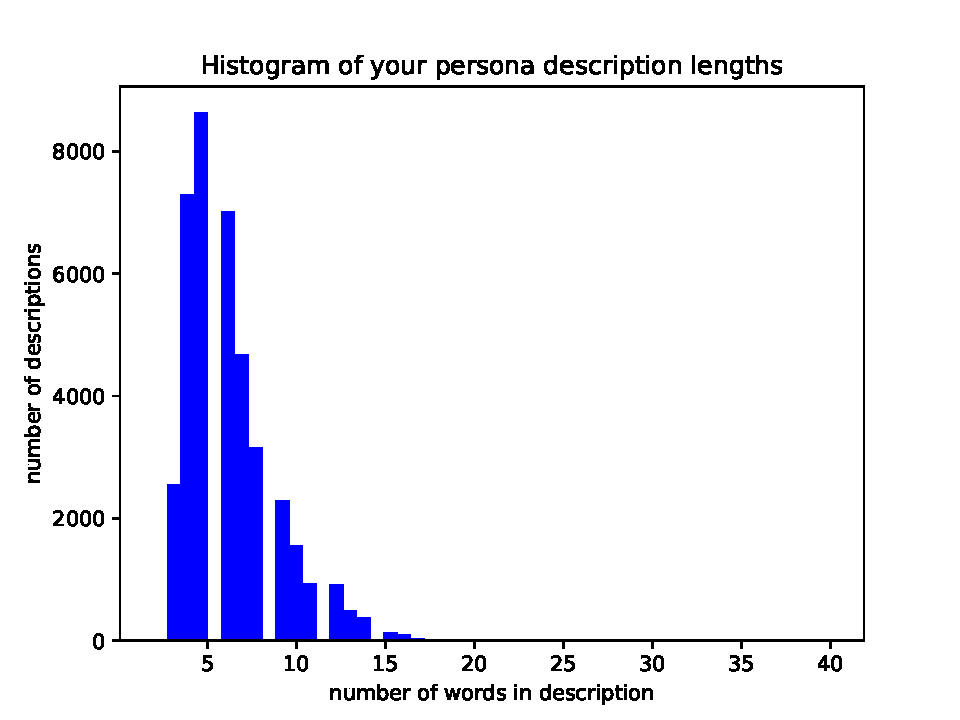
\includegraphics[width=0.5\textwidth]{figures/persona_desc.pdf}
  \caption{Histogram of persona description lengths.}
  \label{fig:histogram_persona_desc}
\end{figure}

\begin{figure}
  \centering
  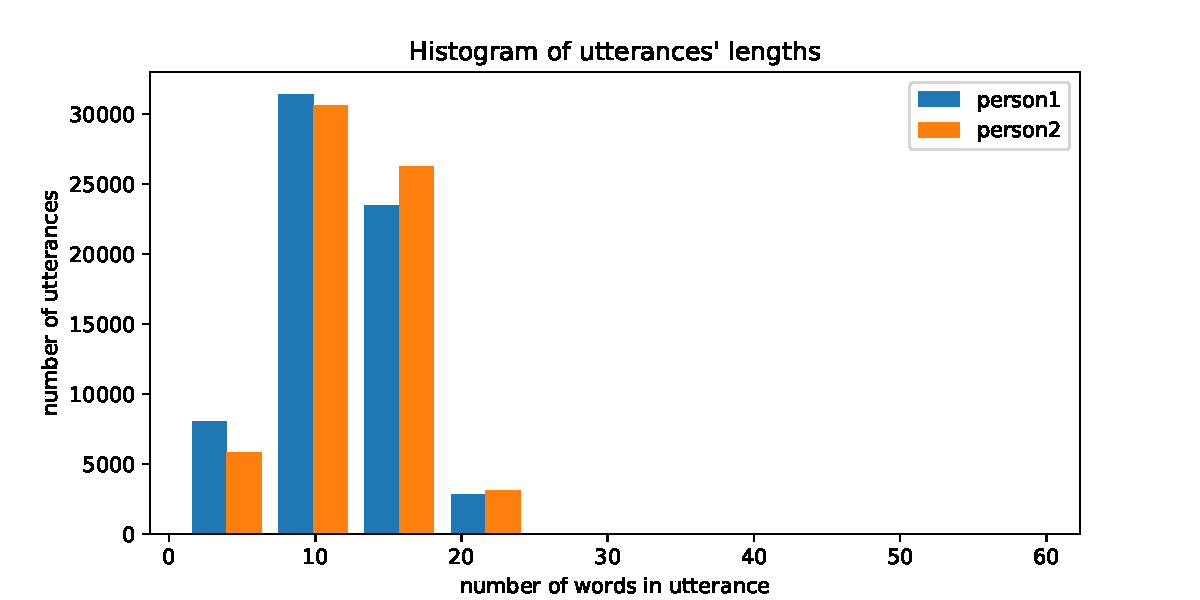
\includegraphics[width=0.5\textwidth]{figures/uttr_length.pdf}
  \caption{Histogram of sequences' lengths of a person.}
  \label{fig:histogram_uttr_length}
\end{figure}

Persona-Chat models normal conversation when 2 people meet for the first meet and try to get know each other better. The aim of the dialogue is to learn about interests of another person, find common ground and discuss their hobbies. The task involves both asking and answering questions. 

Persona-Chat dataset consists of small conversations between 2 crowdworkers from Amazon Mechanical Turk who were randomly paired and asked to act the part of a given provided persona (randomly assigned, and created by another set of crowdworkers). The data collection consists of persona chat (each dialogue has 6-8 turns), personas (set of 1155 possible personas, each consisting of at least 5 profile sentences), revised personas to avoid word overlap, because crowdworkers sometimes could repeat profile information in a chat (the Table \ref{tab:persona_revised}). In turn-based dialogue each message consists of a maximum of 15 words. All statistics are presented in the Table \ref{tab:persona_chat_statistics}, the Figure \ref{fig:histogram_persona_desc} and the Figure \ref{fig:histogram_uttr_length}. An example of Persona-Chat dialogue is shown in the Table \ref{tab:persona_chat}. The dataset contains 262,848 message-responses pairs.

\section{Datasets for stylisation and pre-training} \label{stylistic_dataset_section}
\textbf{Stanford Sentiment Treebank (SST)} contains sentences from movie reviews and includes labels for every syntactically plausible phrase in thousands of sentences. This corpus represents sentiment of reviews. To create SST the corpus of movie review excerpts from the paper \cite{pang2005seeing} is used, where HTML tags and sentences that are not in English are deleted from this dataset. The Stanford Parser is used to parse all 10,662 sentences and some snippet were splitted into multiple sentences. The resulting 215,154 phrases were labeled by Amazon Mechanical Trunk. There are 25 different labels from \textit{very negative} to \textit{very positive}. In this thesis negative and somewhat negative classes are used as one negative class and positive, somewhat positive classes as one positive class. A histogram for positive and negative classes is represented in the Figure \ref{fig:sst}.

\begin{figure}[hb]
  \centering
  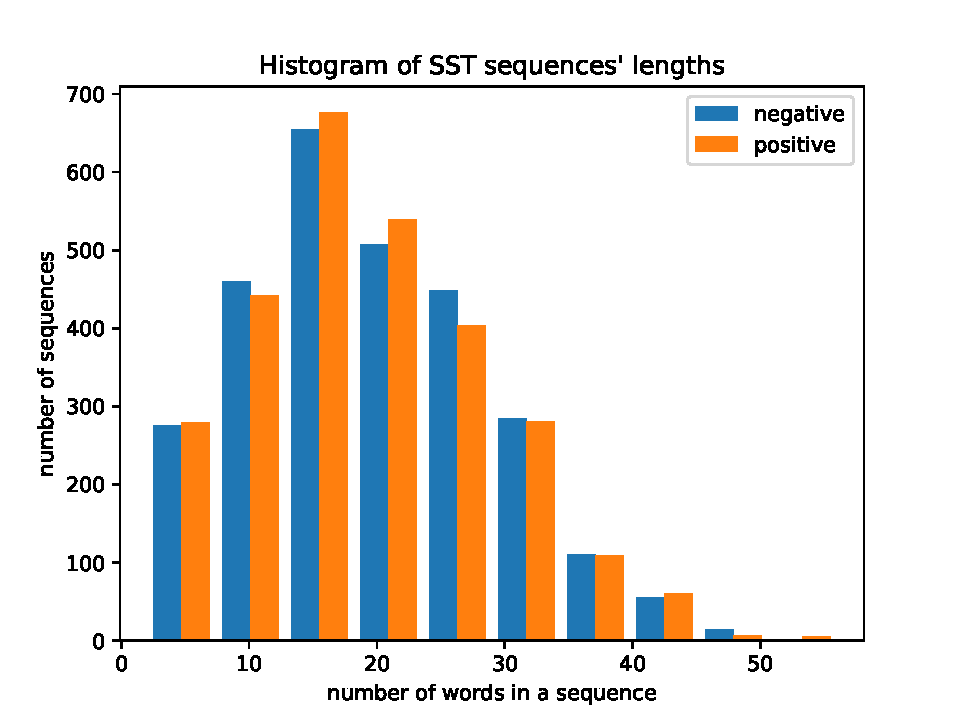
\includegraphics[width=0.5\textwidth]{figures/sst.pdf}
  \caption{Histogram of Stanford Sentiment Treebank labeled reviews.}
  \label{fig:sst}
\end{figure}

For poetic style the \textbf{Shakespeare} dataset was used, which contains all of Shakespeare's plays. A histogram for this dataset is shown in the Figure \ref{fig:shakespeare}.

\begin{figure}[H]
  \centering
  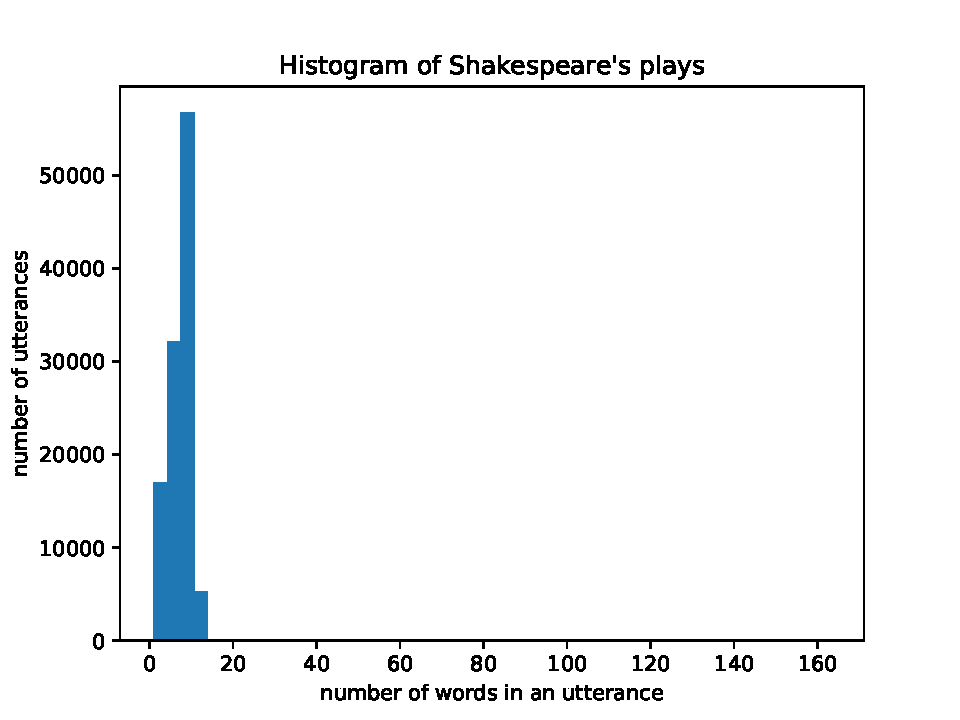
\includegraphics[width=0.5\textwidth]{figures/shakespeare.pdf}
  \caption{Histogram of Shakespeare's plays.}
  \label{fig:shakespeare}
\end{figure}

A dataset of \textbf{english plaintext jokes} was used for generating text with humor style. There are about 208 000 jokes scraped from 3 sources (Table \ref{tab:jokes}). stupidstuff.json is scrapped from stupidstuff.org, wocka.jsom from \url{http://wocka.com}, reddit\_jokes.json is scraped from \url{https://www.reddit.com/r/Jokes} and contains all submissions to the subreddit as of 13.02.2017. A histogram for the dataset is shown in the Figure \ref{fig:jokes}.

\begin{table}[H]
\centering
 \begin{tabular}{|p{4cm}|p{3cm}|p{3cm}|} 
 \hline
 reddit\_jokes.json & 195K jokes & 7.40M tokens \\
 \hline
 stupidstuff.json & 3.77K jokes & 396K tokens \\
 \hline
 wocka.json & 10.0K jokes & 1.11M tokens \\
 \hline
 TOTAL & 208K jokes & 8.91M tokens \\
 \hline
 \end{tabular}
 \caption{Statistics of jokes' dataset.}
\label{tab:jokes}
\end{table}

\begin{figure}[H]
  \centering
  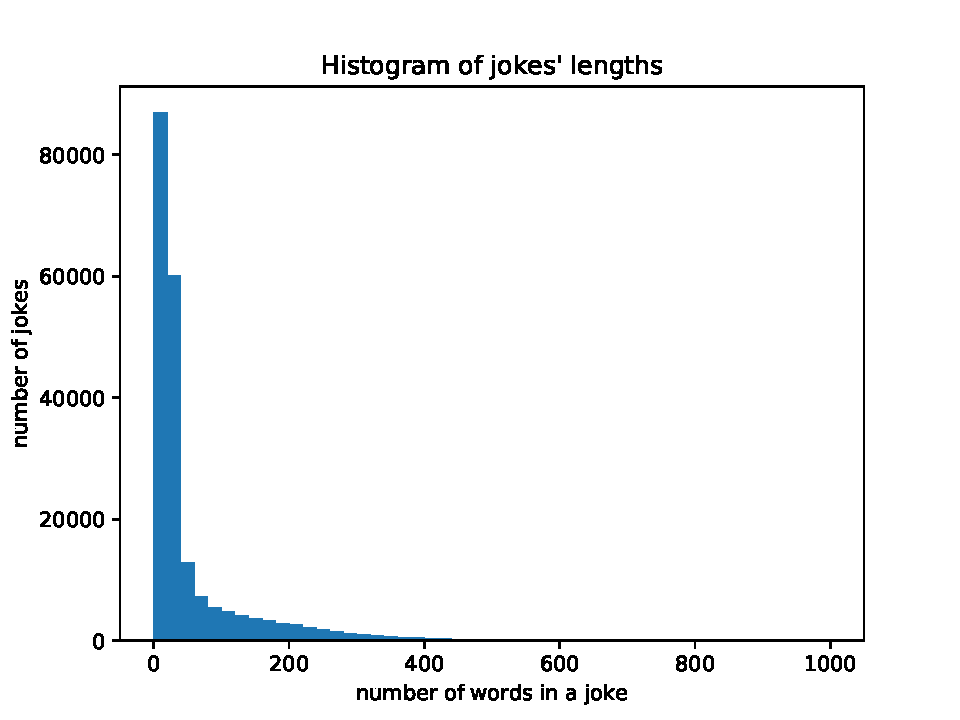
\includegraphics[width=0.5\textwidth]{figures/jokes.pdf}
  \caption{Histogram of jokes lengths.}
  \label{fig:jokes}
\end{figure}

\begin{figure}[H]
  \centering
  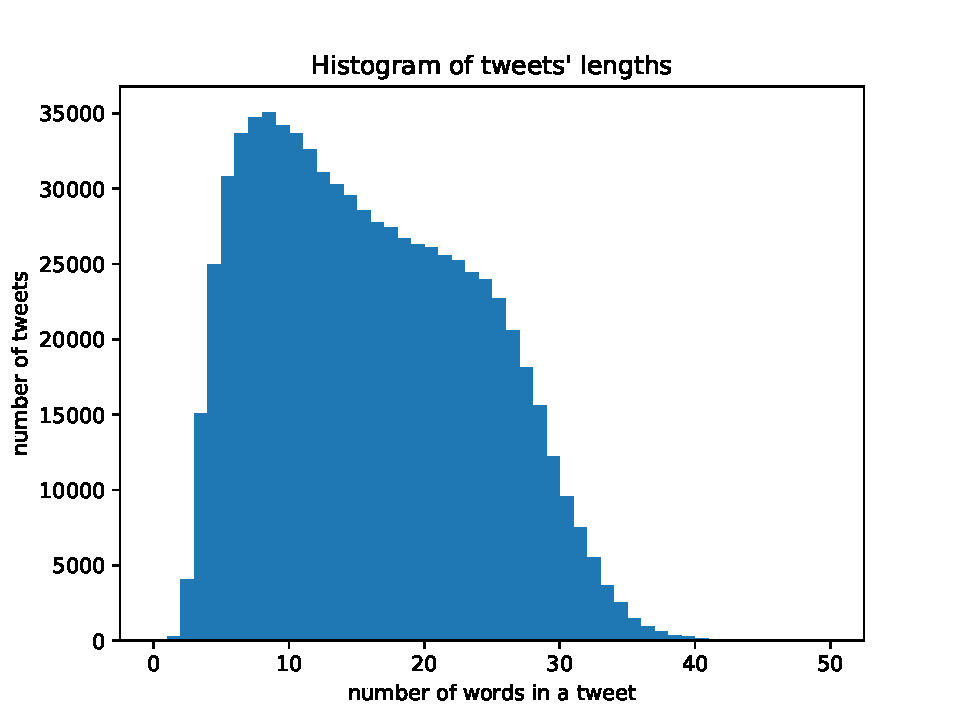
\includegraphics[width=0.5\textwidth]{figures/tweet.pdf}
  \caption{Histogram of tweets' lengths.}
  \label{fig:tweet}
\end{figure}

\textbf{Twitter} dataset contains 867,710 message-response pairs from Twitter and is used for pre-training baseline model. A histogram for the dataset is shown in the Figure \ref{fig:tweet}.

\section{Evaluation methods}\label{eval}
The majority of NLG researches published between 2005-2014 relies on automatic metrics \cite{gkatzia2015snapshot}. A lot of NLG evaluations use automatic metrics, mostly because it is a cheap and fast method. These metrics are reasonable if they are known to be enough correlated with human preferences. According to \cite{artstein2009semi} conversational dialogue systems cannot be evaluated by automatic metrics, because dialogue is heavily dependent on context and theory of current dialogue is not precise enough to predetermine the target output.  

In \cite{novikova2017we} the weak correlation between human and automatic evaluations is also confirmed. Authors compared different word-based (relies on ground-truth references) and grammar-based metrics (does not rely on ground-truth references). Their model, combination of WBMs and GBMs, achieved high correlation with humans but only within a single domain.

Word-based metrics METEOR \cite{banerjee2005meteor}, BLEU \cite{papineni2002bleu}, ROUGE \cite{lin2004rouge} are usually used for automatic summarization. They assume that valid responses have significant word overlap with the ground truth responses. In dialogue systems these metrics cannot be used, because there is significant diversity in the space of valid responses to a given context \cite{liu2016not}.

Grammar-based metrics have been explored in machine translation \cite{gimenez2008smorgasbord} or grammatical error correction \cite{napoles2016there}. The Flesch Reading Ease score \cite{flesch1979write} calculates a ratio between the number of characters per sentence, the number of words per sentence, and the number of syllables per word. Designed grammar-scoring functions are presented in the \cite{napoles2016there}. These metrics can be easily manipulated
with grammatically correct and easily readable output that is unrelated to the input.

Best practices for the human evaluation of NLG are represented in \cite{van2019best}. According to these practices it is better to use separate criteria rather than an overall quality assessment. The effect of fatigue (annotators can change their responses due to fatigue) can be reduced by shortening the task. Order of the compared models may also affect annotators. To reduce this effect, presenting the conditions should be in a systematically varied order. There should always be quite a few participants.

\textbf{A/B testing} \cite{kohavi2017online} is used as human evaluation. This method is described as the randomized assignment to the user of two variants: the \textit{control} and the \textit{treatment}. The control variant typically is the existing version, which in this case it is a real dialogue of two people. The treatment variant is the new version being evaluated -- in this case it is a generated dialogue. 

\begin{eqfloat}
\begin{equation} \label{eq:hypergeometric_distribution}
p_X(k) = Pr(X=k) = \frac{\binom{K}{k} \binom{N-K}{n-k}}{\binom{N}{n}}
\end{equation}
\caption{Hypergeometric distribution, where $N$ is the population size, $K$ is the number of success states in the population, $n$ is the quantity drawn in each trial, $k$ is the number of observed successes. $\binom{n}{k} = \frac{n\,!}{k\,!(n-k)\,!}$ is a binomial coefficient.}
\end{eqfloat}

\textbf{Fisher's exact test} \cite{fisher1922interpretation} is carried out to check human evaluation for statistically significant biases in it. This test is used when there are two nominal variables (nominal variables classify observations into discrete categories) to know if the values of one variable differ among the values of another variable. In this case it is controlled if the order of the dialogs affects the user. 
Fisher's exact test is used when the total sample size is less than 1000. The null hypothesis is that the one variable is independent of the second variable. To confirm or refute this hypothesis, it is necessary to calculate the probability of getting the observed data, and all data sets with more extreme deviations, under the null hypothesis. Hypergeometric distribution (Equation \ref{eq:hypergeometric_distribution}) is used to calculate the probability. If the probability is less than 5\%, the null hypothesis is rejected. 

\chapter{Proposed model design} \label{solution_design}
This chapter describes the proposed model for stylized text generation in dialogue systems and performed experiments. All experiments can be divided into 3 parts: decoding strategies, feature-based decoding modifications and weighted decoding of a combination of language models. The designed architecture for WD of a language models combination is represented in the Figure \ref{architecture_nlg} and implemented in two variants. First variant uses a LSTM-based baseline model. The second one uses pre-trained transformer-based models. For feature-based decoding modifications only encoder-decoder model is used.

\begin{figure}[hbt]
  \centering
  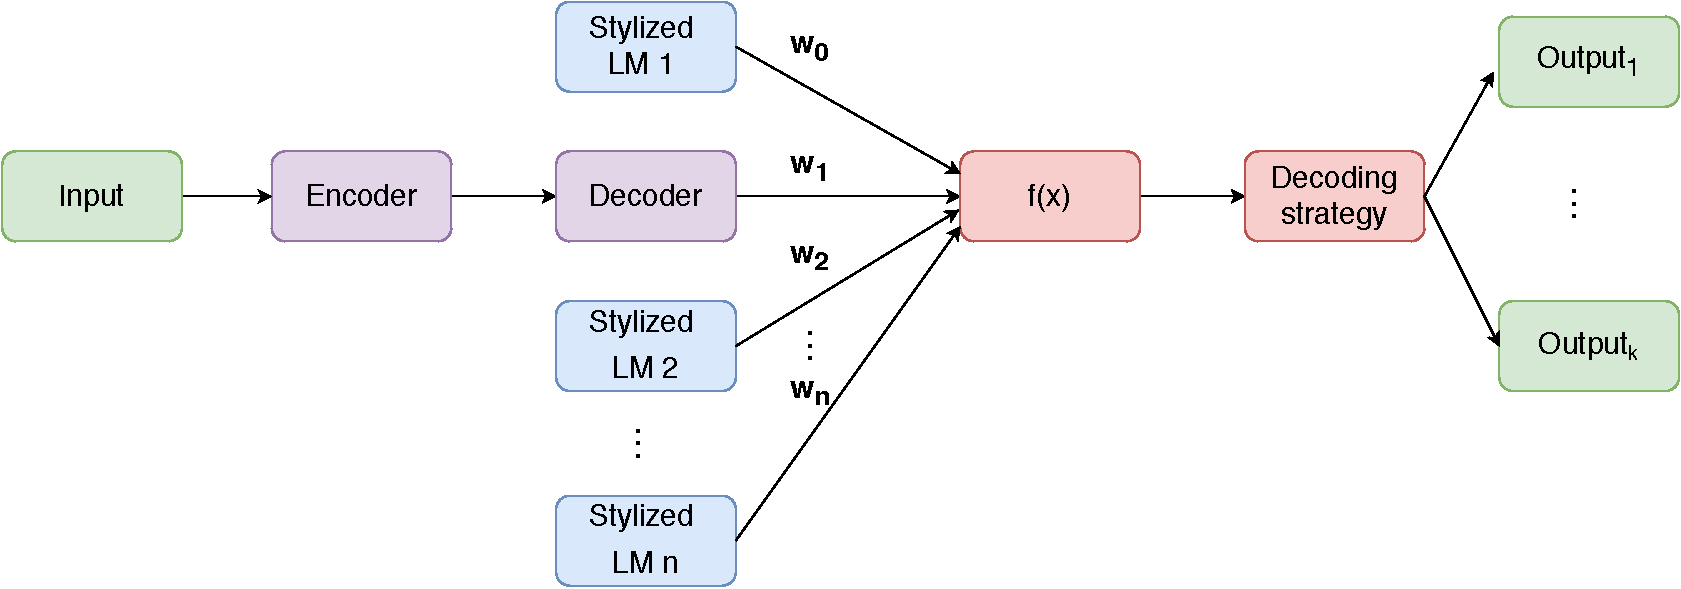
\includegraphics[width=0.8\textwidth]{figures/model.pdf}
  \caption{An architecture of combination models for stylized Natural Language Generation. $w_n$ is a hyperparameter.}
  \label{architecture_nlg}
\end{figure}

An experiment with decoding strategies uses Beam search and Nucleus sampling methods. These decoding strategies, described in detail in the section \ref{decoding_strategies_section}, allow the generation of less generic and repetitive sequences, which affects the user's perception of the text.

\subsubsection{Controlling specificity experiment}
Specificity can make the conversation more informative, because a response like ``I have no idea`` is very general and trivial. NIDF metric, described in the chapter \ref{related_work}, is used as feature-based modification. This approach makes generated text more specific. NIDF represents a measure of word rareness and on each step of the decoding, the probability of each word in the vocabulary is updated in proportion to its rareness. This metric represents a weight for each logarithmic word probability from the encoder-decoder model.

\subsubsection{Length control}
Person's style is represented not only by words, but also by the length of sentences. Some people are used to writing very briefly, and someone likes to paint every detail in a text. Length control is used as feature-based modification.

\subsubsection{Stop words blocking}
Blocking stop words is another feature-based decoding modification. During the decoding data are filtered. In NLP a set of commonly used words in any language is referred to as stop words (for example, ``a'', ``the'', ``I'' etc.). This approach could help to generate more unusual sequences, for example, instead of ``I think'' to use the phrase ``In my opinion''.

\begin{equation} \label{eq:baseline}
p(y_1, ... , y_{T'}|x_1, ... , x_T) \propto \prod_{t=1}^{T'} [w_1 * \log p_1(y_t|x_1, ... , x_T, y_1, ... , y_{t-1}) + \sum_{i=2}^n w_i * \log p_i(y_t| y_1, ... , y_{t-1})]
\end{equation}

The Equation \ref{eq:baseline} is a formal description of the experiment with weighted decoding (Figure \ref{architecture_nlg}), where $x_1, ... , x_T$ is an input sequence and $y_1, ... , y_{T'}$ is its corresponding output sequence whose length $T'$ may differ from $T$. $p_1(y_t|x_1, ... , x_T, y_1, ... , y_{t-1})$ is a distribution from encoder-decoder language model. $p_i(y_t|y_1, ... , y_{t-1})$ is a distribution from each stylized language model, $n$ is a number of stylized models. All distributions are multiplied by a corresponding weight $w$, a hyperparameter in range [0,1] to be chosen. The sum of all weights must be 1.

An experiment of switching BART and GPT-2 models is carried out because text generation using GPT-2 model is independent of the input sequence. Therefore, first a few words are generated using the BART model, and a few using the GPT-2 model. 

\begin{table}[ht]
\centering
 \begin{tabular}{|p{15cm}|} 
 \hline
  i like to remodel homes . \# i like to go hunting . \# i like to shoot a bow . \# my favorite holiday is halloween . CC  SS hi , how are you doing ? i am getting ready to do some cheetah chasing to stay in shape . \# you must be very fast . hunting is one of my favorite hobbies . \# i am ! for my hobby i like to do canning or some whittling . \# \\
 \hline
 \end{tabular}
 \caption{Example of input to the enocder-decoder model, where \# is a sentence delimiter, CC is a delimiter marking the end of a person’s description, SS is a delimiter marking start of a conversation.}
\label{tab:persona_input}
\end{table}

Encoder-decoder model in baseline and pre-trained models is trained on the Persona-Chat dataset, described in the subsection \ref{persona_chat_subsec}. As the input $x$ to the encoder-decoder model, the entire dialogue history, separated by unique token, is used (Table \ref{tab:persona_input}).

Each stylized language model is trained separately on the corresponding stylistic dataset described in the subsection \ref{stylistic_dataset_section}.

\section{Baseline}
Encoder-decoder model in baseline is implemented as LSTM sequence-to-sequence language model, represented in the chapter \ref{nlg_models}, with Luong attention, described in the section \ref{sec_luong}. In the Luong attention, concatenation is used as a score. This model is pre-trained on message-response pairs from Twitter dataset (subsection \ref{stylistic_dataset_section}). Stylized language model is implemented as LSTM-based RNN model.

\section{Pre-trained models}
Combination of BART and GPT-2 models is used to improve results of the created architecture (Figure \ref{architecture_nlg}). BART is an autoencoder for pre-training sequence-to-sequence models, described in the section \ref{bart_section}. BART model with 400M hyperparameters has 12 encoder and decoder layers. This model is chosen because it achieves state-of-the-art results on Conv AI2 task (a dialogue response generation task, conditioned on context and a persona). GPT-2 is a large transformer-based language model, which was trained to predict the next word in 40GB of Internet text. GPT-2 with 117M hyperparameters has large improvements on WikiText2 dataset for language modelling. This model is a successor to GPT, described in the section \ref{sec_gpt} and used as stylized language model. 

\begin{table}[ht]
\centering
 \begin{tabular}{|p{5cm}|p{3cm}|p{3cm}|} 
 \hline
 \textbf{Model name} & \textbf{Valid F1} & \textbf{Valid PPL} \\
 \hline
 Seq2Seq + Attention & 16.02 & 35.07 \\
 \hline
 BART & 20.72 & 11.85 \\
 \hline
 \end{tabular}
 \caption{BART outperforms previous work on conversational response generation. Results are from \cite{lewis2019bart}. \textbf{PPL} (perplexity) is a measurement of how well a probability model predicts a sample. A low perplexity is good at predicting the sample, because perplexity is just an exponentiation of the entropy. \textbf{F1} is a measure of a test's accuracy. $F1 = \frac{2}{recall^{-1} + precision^{-1}}$, where $recall$ is the number of correct positive results divided by all samples that should have been identified as positive and $precision$ is the number of correct positive results divided by the number of all positive results returned by the model.}
\label{tab:bart_statistic}
\end{table}

\section{Proposed evaluation approach}
There is a lot of research, which shows that human and automatic evaluations have weak correlation (Subsection \ref{eval}). In dialogue systems there are lots of ways how to answer the opponent's correctly, that's why in this thesis only human evaluaton is used. 

A/B tests were used for human evaluation. Several manifestations of human styles were evaluated, such as sentiment (positive, negative), poetry, humor, and specificity. Users were given a questionnaire with several questions (``Which dialogue is more positive?'', ``Which dialogue is more negative?'', ``Which dialogue is more poetic?'', etc.) and for each question there were 2 dialogs as answer options. One of the dialogs was generated by the model, and the second one was from real life.

For the Fisher's exact test, 2 questionaire were created, where there was only 1 question (``Which dialogue is more poetic?''). In the first case, as a response option, the generated dialogue was first given and then the real dialogue, and in the second, vice versa.

\chapter{Implementation} \label{chap_implementation}
All parts of the architecture proposed in the Figure \ref{architecture_nlg} were implemented in Python 3.7.3 with using PyTorch 1.4.0 framework.

\subsubsection{Implementation details of the experiments}
In the length control experiment at each iteration, when generating the next word, a small weight is added to the logarithmic probability of the \texttt{[EOS]} (end of sequence) symbol. 

For the experiment with stop words blocking, stop words are used from NLTK\protect\footnotemark (suite of libraries and programs for symbolic and statistical NLP). During decoding in each iteration, when selecting the next word in the sequence, it is checked if this word is not contained in stop words. If word is in stop words, a logarithmic probability for this word is set to 0. 

In the experiment with switching models, $n$ words in a sequence are generated over encoder-decoder model and $n$ words are generated over stylized language model, $n$ is a hyperparameter. Sequence generation stops when the end mark of the sequence is generated or the length of the sequence is equal to the maximum length. 

\footnotetext{\url{https://www.nltk.org/}}

\subsubsection{Data processing}
For training language models several datasets are splitted. Persona-Chat is splitted into train data -- 70\%, valid data -- 20\% and test data -- 10\%. For SST dataset annotators most often used only 5-class classification: negative, somewhat negative, neutral, positive or somewhat positive. Many of sentences could be considered neutral, therefore, to generate text with positive and negative sentiment I have used negative and somewhat negative classes as one negative class and positive, somewhat positive classes as one positive class. Twitter dataset is splitted into train data -- 85\%, valid data -- 10\% and test data -- 5\%.

Data are tokenized, where tokenization is a process of splitting text into units represented at model's input and replacing sensitive data with unique identification symbols that retain all the essential information about the data without compromising its security. Spacy\protect\footnotemark library is used with few handcrafted rules for tokenization. As input GloVe (Global Vectors) embeddings are used for distributed word representation \cite{pennington2014glove}. It is a model, which maps words into a meaningful space where the distance between words is related to semantic similarity. Outputs of encoder-decoder and stylized language models (logarithmic probabilities of words) are multiplied by weights (weight is a hyperparameter to be chosen) to increase or decrease the probability of words and finally these outputs are added up.

\footnotetext{\url{https://spacy.io/}}

\begin{eqfloat}
\begin{equation} \label{eq:cross_entropy}
H(p,q) = -\sum_{x \in X} p(x)\log q(x)
\end{equation}
\caption{$p$ is the target distribution, $q$ is the approximation of the target distribution. $p(x)$ is the probability of the event $x$ in $p$, $q(x)$ is the probability of the event $x$ in $q$.}
\end{eqfloat}

\subsubsection{Implementation details of the baseline model}
For all experiments with the baseline 2-layer LSTMs were used in both the encoder and decoder with 512 hidden unites in each hidden layer. A dropout \cite{srivastava2014dropout} was used with the probability of $50\%$ to prevent neural networks from overfitting. \textit{Cross-entropy} (measure of the difference between 2 probability distributions for a given random variable or set of events) was used as a loss function. Formally representation of cross-entropy is in the Equation \ref{eq:cross_entropy}. \textit{Adam} \cite{kingma2014adam} was used as the optimization algorithm.


\subsubsection{Implementation details of the pre-trained model}
For BART and GPT-2 model is used Byte Pair Encoding \cite{sennrich2015neural}. In the BART model, the learning rate \cite{jacobs1988increased} was set to $3\mathrm{e}{-5}$, label smoothing \cite{szegedy2016rethinking} was 0.1, dropout was also 0.1. BART decoder is an equivalent to the GPT model, described in the section \ref{sec_gpt}. GPT-2 is a direct scale-up of GPT, with more parameters (1.5 billion parameters) and trained on more amount of data. GPT-2 model uses more words in a vocabulary than GPT, what means that before a combination of these models, it is necessary to convert a distribution of logarithmic probabilities of the next word in a sequence over all the words in the smallest vocabulary to the distribution over the biggest one and add 0 if the word does not exist. Outputs of BART model, transformed to GPT-2 vocabulary, and logarithmic probabilities of words of GPT-2 models are multiplied by weights to increase or decrease the probability of words and finally these outputs are added up.

Each GPT-2 model represents one style. 4 such models were fine-tuned for humor, positive and negative sentiment and poetic style. The model was trained with batch size parameter set to 1, learning rate for Adam is $1\mathrm{e}{-4}$, 50000 chars was a minimum size to concatenate input files with \texttt{<|endoftext|>} separator. 

\subsubsection{Evaluation details}
To evaluate the dialogues, 30 people participated with the year of birth in the range from 1991 to 2004 with different levels of education and field of activity. For the Fisher's exact test, 7 people were recruited for one questionaire and 8 other people for another. 

\chapter{Results and discussion} \label{results_discuss}
In this chapter, the results of the experiments described in the previous section are presented and their implications are discussed. Human evaluation occurred only for those experiments that were subjectively considered more successful.

All experiments with features, decoding strategies and combination of models are carried out on pre-trained models, because the dialogs generated by the baseline model do not make sense in the context. The example in the Table \ref{tab:baseline_experiment} shows that the model also has a repetition problem, such as repetition of the part of a sequence (``I am``), repetition of phrases (``I am afraid``). These problems can be because of the small amount of data and LSTM neural networks still have a problem to hold a context. In comparison with the baseline model, the dialogue generated using the BART model (Table \ref{tab:bart_experiment}) is more logical and diverse.

\begin{table}[ht]
\centering
 \begin{tabular}{|p{14cm}|}
 \hline
 \textbf{Person 1 description:} 1. as a child, i won a national spelling bee. 2. i have been published in the new yorker magazine. 3. i am a gourmet cook. 4. i have perfect pitch. \\
 \hline
 \textbf{Person 2 description:} 1. i am very athletic. 2. i wear contacts. 3. i have brown hair. 4. i love bicycling. 5. i hate carrots. \\
 \hline
 \textbf{Person1:} i am afraid. \\
 \textbf{Person2:} i am a business employee.  \\ 
 \textbf{Person1:} i am a surfer. \\
 \textbf{Person2:} i am not much of a foodie. \\
 \textbf{Person1:} i am afraid. \\
 \textbf{Person2:} that is cool. \\
 \textbf{Person1:} i do. i like to starve. \\
 \textbf{Person2:} i like to go to the homeless. \\
 \textbf{Person1:} i am not really a fan of harry potter. \\
 \textbf{Person2:} i am good. i am in tampa. \\
 \textbf{Person1:} i am from boston ma. \\
 \textbf{Person2:} i am in boston. \\
 \hline
 \end{tabular}
 \caption{Example of a dialogue conversation generated by baseline model with Beam search decoding strategy.}
\label{tab:baseline_experiment}
\end{table}

\begin{table}
\centering
 \begin{tabular}{|p{14cm}|}
 \hline
 \textbf{Person 1 description:} 1. as a child, i won a national spelling bee. 2. i have been published in the new yorker magazine. 3. i am a gourmet cook. 4. i have perfect pitch. \\
 \hline
 \textbf{Person 2 description:} 1. i am very athletic. 2. i wear contacts. 3. i have brown hair. 4. i love bicycling. 5. i hate carrots. \\
 \hline
 \textbf{Person1:} hi, how are you doing today?  \\
 \textbf{Person2:} that is cool. I am a chef  \\ 
 \textbf{Person1:} i don't like carrots either. I am a gourmet cook. \\
 \textbf{Person2:} i am very athletic. i love to play sports \\
 \textbf{Person1:} i ride my bike to work as well. \\
 \textbf{Person2:} that is awesome. i am very athletic, so i love spelling \\
 \textbf{Person1:} i have been published in a new yorker magazine \\
 \textbf{Person2:} that is cool. i have never heard of it \\
 \textbf{Person1:} i do not make any spelling mistakes\\
 \textbf{Person2:} that is great! \\
 \textbf{Person1:} i am from california. my hair is brown \\
 \textbf{Person2:} what is your ethnicity? i am asian. \\
 \hline
 \end{tabular}
 \caption{Example of a dialogue conversation generated by BART model with Beam search decoding strategy.}
\label{tab:bart_experiment}
\end{table}

Results of using beam search and Nucleus sampling methods are shown in the Tables \ref{tab:beam_search} and \ref{tab:nucleus_sampling}. All these decoding strategies are described in detail in the section \ref{decoding_strategies_section}.

\begin{table}
\centering
 \begin{tabular}{|p{14cm}|} 
 \hline
 \textbf{Person 1 description:} 1. as a child, i won a national spelling bee. 2. i have been published in the new yorker magazine. 3. i am a gourmet cook. 4. i have perfect pitch. \\
 \hline
 \textbf{Person 2 description:} 1. i am very athletic. 2. i wear contacts. 3. i have brown hair. 4. i love bicycling. 5. i hate carrots. \\
 \hline
 \textbf{Person1:} hi , how it goes \\
 \textbf{Person2:} i love you. \\
 \textbf{Person1:} i do not love you. What do you mean? \\
 \textbf{Person2:} i am very glad you came to England \\
 \textbf{Person1:} that sounds like a good man \\
 \textbf{Person2:} i have not heard of you yet. \\
 \textbf{Person1:} i have been, i have been. You are welcome, sir \\
 \hline
 \end{tabular}
 \caption{Experiment of Beam search decoding method with poetic style.}
\label{tab:beam_search}
\end{table}

\begin{table}
\centering
 \begin{tabular}{|p{14cm}|} 
 \hline
 \textbf{Person 1 description:} 1. as a child, i won a national spelling bee. 2. i have been published in the new yorker magazine. 3. i am a gourmet cook. 4. i have perfect pitch. \\
 \hline
 \textbf{Person 2 description:} 1. i am very athletic. 2. i wear contacts. 3. i have brown hair. 4. i love bicycling. 5. i hate carrots. \\
 \hline
 \textbf{Person1:} hi, how is thy name \\
 \textbf{Person2:} i am an ass, and thou shalt be \\
 \textbf{Person1:} i am sure you have not seen a man till you \\
 \textbf{Person2:} i do not know, Wherefore you speak. \\
 \textbf{Person1:} i ride you, And i love it \\
 \textbf{Person2:} i am very glad you are come \\
 \textbf{Person1:} i have a daughter of old \\
 \hline
 \end{tabular}
 \caption{Experiment of Nucleus sampling decoding method with poetic style.}
\label{tab:nucleus_sampling}
\end{table}

In the experiment using the Nucleus sampling, a lot more poetic old-fashioned phrases (``thy name``, ``thou shalt be``, ``Wherefore``) were generated than using Beam search strategy (``You are welcome, sir``). In this experiment, both strategies have a problem with the context; the generated sequences are not very interconnected.

\section{Feature-based decoding modifications}
\subsubsection{Controlling specificity}
In the experiment the Normalized Inverse Document Frequency feature is used as a decoding feature. This approach makes generated text more specific, because the less often a word is found in a dataset the more weight is set for the word probability. 

\begin{table}[ht]
 \begin{tabular}{|p{14cm}|}
 \hline
 \textbf{Person 1 description:} 1. as a child, i won a national spelling bee. 2. i have been published in the new yorker magazine. 3. i am a gourmet cook. 4. i have perfect pitch. \\
 \hline
 \textbf{Person 2 description:} 1. i am very athletic. 2. i wear contacts. 3. i have brown hair. 4. i love bicycling. 5. i hate carrots. \\
 \hline
 \textbf{Person1:} (Silence) \\
 \textbf{Person2:} hello , how are you doing today? \\ 
 \textbf{Person1:} hi! i work as a gourmet cook \\
 \textbf{Person2:} what kind of gourmet cook do you cook?\\
 \textbf{Person1:} i do not like carrots. i throw them away.\\
 \textbf{Person2:} what kind of carrots do you discard? \\
 \textbf{Person1:} really. but, i can sing pitch perfect.\\
 \textbf{Person2:} what kind of music do you sing pitch perfect?\\
 \textbf{Person1:} i also cook, and i ride my bike to work.\\
 \textbf{Person2:} that sounds fun! i ride my bike to work as well. \\
 \textbf{Person1:} great! i had won an award for spelling bee. \\
 \textbf{Person2:} awesome! what kind of spelling bee did you win?\\
 \hline
 \end{tabular}
\caption{Generated conversation by BART model with specifity, weight = 5.}
\label{tab:bart_nidf}
\end{table}

The experiment of using BART model with NIDF is shown in the Table \ref{tab:bart_nidf}. NIDF is multiplied by hand tuned weight to increase the probability of words. The conversation generated by BART model with NIDF uses such specific words as ``discard'', ``award'' and \textbf{64.3\%} of people consider that the generated dialogue is more specific than real one (Table \ref{tab:persona_chat}). The results of the specificity control experiment with different weights are represented in the Tables \ref{tab:bart_conversation_idf-5_ap}, \ref{tab:bart_conversation_idf10_ap}, \ref{tab:bart_conversation_idf-10_ap}. The experiments showed that the greater the weight, the more rare words are generated, but the dialogue at the same time turns out to be meaningless.

\subsubsection{Length control}
\begin{table}[ht]
\centering
 \begin{tabular}{|p{2cm}|p{6cm}|p{6cm}|} 
 \hline
 \multicolumn{3}{|p{14cm}|}{\textbf{Person 1 description:} 1. as a child, i won a national spelling bee. 2. i have been published in the new yorker magazine. 3. i am a gourmet cook. 4. i have perfect pitch. }\\
 \hline
 \multicolumn{3}{|p{14cm}|}{\textbf{Person 2 description:} 1. i am very athletic. 2. i wear contacts. 3. i have brown hair. 4. i love bicycling. 5. i hate carrots.} \\
 \hline
 \textbf{Person1:} & hi, how are you tonight? & hi, how are you?\\
 \hline
 \textbf{Person2:} & i am a chef. i love to cook. & i am a chef. \\
 \hline
 \textbf{Person1:} & i do not like carrots either..... & i do not like carrots\\
 \hline 
 \textbf{Person2:} & i am very athletic. i ride my bike to work every morning & i am very athletic\\
 \hline 
 \textbf{Person1:} & i am from the country of birth & i am from texas\\
 \hline
 \end{tabular}
 \caption{Experiment of generated sequences with specified length.}
\label{tab:set_len}
\end{table}
For this experiment 2 lengths of a sequence were chosen: 5 and 20 words. Generated sequences with this feature are shown in the Table \ref{tab:set_len}. \textbf{71.4\%} people consider, that dialogues generated with a lot of words in a sentence are more interesting, even though long sequences have a punctuation problem. In some cases, when a full stop (``.``) was generated, but the maximum sequence length was not yet reached, the model continued to generate full tops further, for example, as in the sentence ``i do not like carrots either.....``. Another experiment with the length control is shown in the Table \ref{tab:bart_length_control}. Short sentences in the experiments are not perceived by people as one dialogue, but rather, as separate expressions.

\subsubsection{Stop word blocking}
\begin{table}[H]
\centering
 \begin{tabular}{|p{14cm}|} 
 \hline
 \textbf{Person 1 description:} 1. as a child, i won a national spelling bee. 2. i have been published in the new yorker magazine. 3. i am a gourmet cook. 4. i have perfect pitch. \\
 \hline
 \textbf{Person 2 description:} 1. i am very athletic. 2. i wear contacts. 3. i have brown hair. 4. i love bicycling. 5. i hate carrots. \\
 \hline
 \textbf{Person1:} good morning \\
 \textbf{Person2:} oh yeah \\
 \textbf{Person1:} oh yeah \\
 \textbf{Person2:} oh nice sound \\
 \textbf{Person1:} awwwwwwwwwwwwwww \\
 \hline
 \end{tabular}
 \caption{Experiment of a generated dialogue with blocking stop words.}
\label{tab:stop_words}
\end{table}
An example of the blocking stop words experiment is illustrated in the Table \ref{tab:stop_words}. Represented results show that generated sequences are very generic, have a repetition problem (``oh yeah``) and don't make sense in a context. For this experiment, there was no human evaluation.

\section{Weighted decoding of combination BART and GPT-2 models}
Results of this experiment are generated dialogues from combination of BART and GPT-2 models for stylization, the weights for other stylistic language models are set to 0.

Example of a generated dialogue with humor is shown in the Table \ref{tab:combo_bart_gpt2_jokes}. The weight for encoder-decoder model is set to 0.3, the weight for stylized language model is set to 0.7. These hyperparameters were manual tunned. Compared to the generated dialogue using only the BART model (Table \ref{tab:bart_experiment}), this conversation is not very different, although, for example, the phrase: ``i am a chef for carrots'' may seem rather funny, because the opponent does not like carrots and \textbf{57.14\%} people consider that this dialogue is comical.

\begin{table}[H]
\centering
 \begin{tabular}{|p{14cm}|} 
 \hline
 \textbf{Person 1 description:} 1. as a child, i won a national spelling bee. 2. i have been published in the new yorker magazine. 3. i am a gourmet cook. 4. i have perfect pitch. \\
 \hline
 \textbf{Person 2 description:} 1. i am very athletic. 2. i wear contacts. 3. i have brown hair. 4. i love bicycling. 5. i hate carrots. \\
 \hline
 \textbf{Person 1:} hey! how are you today? \\ 
 \textbf{Person 2:} hi! i work as a gourmet cook \\
 \textbf{Person 1:} i was just about to go to a gourmet cook shop. \\
 \textbf{Person 2:} i do not like carrots. i throw them away. \\
 \textbf{Person 1:} i am a chef for carrots.\\
 \textbf{Person 2:} really. but, i can sing pitch perfect. \\
 \textbf{Person 1:} i love the chorus. \\
 \textbf{Person 2:} i also cook, and i ride my bike to work. \\
 \textbf{Person 1:} great! i had won an award for spelling bee.\\
 \textbf{Person 2:} that is awesome. i am sure! \\
 \hline
 \end{tabular}
 \caption{Experiment of weighted decoding of BART with GPT-2 trained on dataset with jokes.}
\label{tab:combo_bart_gpt2_jokes}
\end{table}

Generated dialogue with poetic style is represented in the Table \ref{tab:poetic_shakespear}. Hyperparameters for weighted decoding are set to 0.2 for BART and 0.8 for GPT-2 model. In the example a poetic appeal to a person (``My Lord'') is used, which means a manifestation of style. \textbf{64.3\%} people consider that this dialogue is more poetic than the real one.

\begin{table}[H]
\centering
 \begin{tabular}{|p{14cm}|} 
 \hline
 \textbf{Person 1 description:} 1. as a child, i won a national spelling bee. 2. i have been published in the new yorker magazine. 3. i am a gourmet cook. 4. i have perfect pitch. \\
 \hline
 \textbf{Person 2 description:} 1. i am very athletic. 2. i wear contacts. 3. i have brown hair. 4. i love bicycling. 5. i hate carrots. \\
 \hline
 \textbf{Person1:} (Silence) \\
 \textbf{Person2:} hi there, how shall we get on?  \\ 
 \textbf{Person1:} i love carrots. i know how you feel. \\
 \textbf{Person2:} i do not know what to do, My lord. \\
 \textbf{Person1:} i am not a great singer. \\
 \textbf{Person2:} i ride to work \\
 \textbf{Person1:} that is the same. \\
 \textbf{Person2:} i am not heard of that. \\
 \textbf{Person1:} i am not very good writer, but I am very good poet. \\
 \textbf{Person2:} i am not a spelling student. But i have a question for you. \\
 \textbf{Person1:} i am not a cook, I am a gourmet cook \\
 \textbf{Person2:} i am not a fool. But I am a man of color  \\
 \hline
 \end{tabular}
 \caption{Experiment of weighted decoding of BART and GPT-2 trained on Shakespeare dataset.}
\label{tab:poetic_shakespear}
\end{table}

In the Table \ref{tab:sst_wd} GPT-2 is trained on SST dataset. As a result generated sentences are short. It could be because sentences in the courpus are ranging from 10 to 20 words (a histogram of the SST dataset is in the Figure \ref{fig:sst}). The negative and positive moods are not expressed in the example. Generated dialogues were compared with the real conversation and in case of positive sentiment only \textbf{21.4\%} people consider that generated dialogue is positive, in case of negative sentiment -- \textbf{50\%} people think that generated conversation is more negative than the real one. 

\begin{table}[H]
\centering
 \begin{tabular}{|p{7cm}|p{7cm}|} 
 \hline
 \textbf{Generated conversation with negative SST stylistic dataset.} & \textbf{Generated conversation with positive SST stylistic dataset.}\\
 \hline
 \multicolumn{2}{|p{14cm}|}{\textbf{Person 1 description:} 1. i am very athletic. 2. i wear contacts. 3. i have brown hair. 4. i love bicycling. 5. i hate carrots.} \\
 \hline
 \multicolumn{2}{|p{14cm}|}{\textbf{Person 2 description:} 1. as a child, i won a national spelling bee. 2. i have been published in the new yorker magazine. 3. i am a gourmet cook. 4. i have perfect pitch.} \\
 \hline
 \textbf{Person1:} hi there? & \textbf{Person1:} hi how are you \\
 \textbf{Person2:} i work. &  \textbf{Person2:} i love cooking \\ 
 \textbf{Person1:} i do not eat & \textbf{Person1:} i am not \\
 \textbf{Person2:} i am a singer & \textbf{Person2:} i have you heard \\
 \textbf{Person1:} that is awesome & \textbf{Person1:} that sounds fun. \\
 \textbf{Person2:} that is cool? & \textbf{Person2:} that is pretty?  \\
 \textbf{Person1:} i have not. & \textbf{Person1:} i do you know. \\
 \textbf{Person2:} i have been. & \textbf{Person2:} i am very. \\
 \textbf{Person1:} i do not know & \textbf{Person1:} i am sure. \\
 \textbf{Person2:} i am very good & \textbf{Person2:} i am a professional \\
 \textbf{Person1:} i am white & \textbf{Person1:} i am black \\
 \textbf{Person2:} i am asian & \textbf{Person2:} i am asian \\
 \hline
 \end{tabular}
 \caption{Experiment of weighted decoding of BART and GPT-2 trained on SST stylistic dataset.}
\label{tab:sst_wd}
\end{table}

General conclusion from this experiment is that the more weight was set on generating the style, the more the context began to get lost. Generated sentences were often unrelated in context. Therefore, the following experiment was conducted with the alternate use of models.

\section{Switching BART and GPT-2 models}
In this experiment, alternating the generation of words by the encoder-decoder and stylized language models. $n$ words in a sequence are generated over BART and $n$ words are generated over GPT-2 model, where $n$ is a hyperparameter. Sequence generation stops when the end mark of the sequence is generated or the length of the sequence is equal to the maximum length.

Example of the experiment is represented in the Table \ref{tab:jokes_switch}. When generating sequences, there is still a problem of context, but already the model sometimes generates answers to the opponent's input (``-i love carrots but I hate carrots too. -i don't like it either.''). \textbf{71.4\%} people consider that this dialogue is more comic than the real one.

\begin{table}[H]
\centering
 \begin{tabular}{|p{14cm}|} 
 \hline
 \textbf{Person 1 description:} 1. i am very athletic. 2. i wear contacts. 3. i have brown hair. 4. i love bicycling. 5. i hate carrots. \\
 \hline
 \textbf{Person 2 description:} 1. as a child, i won a national spelling bee. 2. i have been published in the new yorker magazine. 3. i am a gourmet cook. 4. i have perfect pitch. \\
 \hline
 \textbf{Person1:} hi there. how much do you charge?  \\
 \textbf{Person2:} i love carrots but I hate carrots too.  \\ 
 \textbf{Person1:} i don't like it either. \\
 \textbf{Person2:} i am a singer.\\
 \textbf{Person1:} i ride the bike to work. The weather is beautiful  \\
 \textbf{Person2:} i am not sure. i have never seen that. What is the spelling of the word   \\
 \textbf{Person1:} i don't know. \\
 \textbf{Person2:} i am a gourmet chef. \\
 \textbf{Person1:} i am not a spelling bee. \\
 \textbf{Person2:} i am not a cook. What is your favorite food? I would love to know. \\
 \textbf{Person1:} i am a white man \\
 \textbf{Person2:} i am a asian \\
 \hline
 \end{tabular}
 \caption{Experiment of switching BART and GPT-2 models trained on jokes stylistic dataset.}
\label{tab:jokes_switch}
\end{table}

The sentiment and poetic style are not expressed in the examples shown in the Tables \ref{tab:shakespeare_switch}, \ref{tab:sst_switch}. For the conversation generated by the model fine-tuned on the Shakespeare dataset only \textbf{37.5\%} of people consider this dialogue poetic. \textbf{33.3\%} is a human evaluation for negative sentiment and \textbf{23.8\%} is for positive sentiment.

\begin{table}[H]
\centering
 \begin{tabular}{|p{14cm}|} 
 \hline
 \textbf{Person 1 description:} 1. i am very athletic. 2. i wear contacts. 3. i have brown hair. 4. i love bicycling. 5. i hate carrots. \\
 \hline
 \textbf{Person 2 description:} 1. as a child, i won a national spelling bee. 2. i have been published in the new yorker magazine. 3. i am a gourmet cook. 4. i have perfect pitch. \\
 \hline
 \textbf{Person1:} hi , i am jane  \\
 \textbf{Person2:} i love to cook. i am a gourmet. \\ 
 \textbf{Person1:} i do not like carrots. i am allergic \\
 \textbf{Person2:} i am a very athletic young man, and you?\\
 \textbf{Person1:} i ride my bike, but I do fear of heights. \\
 \textbf{Person2:} that is great \\
 \textbf{Person1:} i am a goner  \\
 \textbf{Person2:} i have been published.\\
 \textbf{Person1:} i have done a lot. i am very good  \\
 \textbf{Person2:} i am a chef . is a gourmet too \\
 \textbf{Person1:} i am not sure of my ethnicity \\
 \textbf{Person2:} i am not sure of what that is. \\
 \hline
 \end{tabular}
 \caption{Experiment of switching BART and GPT-2 models trained on Shakespeare dataset.}
\label{tab:shakespeare_switch}
\end{table}

\begin{table}[H]
\centering
 \begin{tabular}{|p{7cm}|p{7cm}|} 
 \hline
 \textbf{Generated conversation with negative SST stylistic dataset.} & \textbf{Generated conversation with positive SST stylistic dataset.}\\
 \hline
 \multicolumn{2}{|p{14cm}|}{\textbf{Person 1 description:} 1. i am very athletic. 2. i wear contacts. 3. i have brown hair. 4. i love bicycling. 5. i hate carrots.} \\
 \hline
 \multicolumn{2}{|p{14cm}|}{\textbf{Person 2 description:} 1. as a child, i won a national spelling bee. 2. i have been published in the new yorker magazine. 3. i am a gourmet cook. 4. i have perfect pitch.} \\
 \hline
 \textbf{Person1:} hi there, how much do you care about? & \textbf{Person1:} hi, who wrote that poem? \\
 \textbf{Person2:} i love to cook, but I do not think i have ever been more captivating &  \textbf{Person2:} i love to cook, and i am ... \\ 
 \textbf{Person1:} i don't like it when the carrots come out & \textbf{Person1:} i don't like, i n't like carrots, i don't like vinegar \\
 \textbf{Person2:} i have a lot of friends & \textbf{Person2:} i am not a great writer. \\
 \textbf{Person1:} i ride the bike of course & \textbf{Person1:} i ride his bike to and from the office. \\
 \textbf{Person2:} i have to be a bit more of a nerd & \textbf{Person2:} that is, i. e. i am not allowed to use it.  \\
 \textbf{Person1:} i have a lot of fun & \textbf{Person1:} i have a lot of fun. \\
 \textbf{Person2:} i have a hard time believing that a movie is that good & \textbf{Person2:} i have a lot of fun. it is one of my all-time favourite books. \\
 \textbf{Person1:} i amiable and kind of sweet & \textbf{Person1:} i am not a spelling mistake \\
 \textbf{Person2:} i am not sure & \textbf{Person2:} i am not a cook, but rather a chef \\
 \textbf{Person1:} i am not sure I can believe it & \textbf{Person1:} i am not a white man, but i am a black man \\
 \textbf{Person2:} i do n't like it & \textbf{Person2:} i am not sure why \\
 \hline
 \end{tabular}
 \caption{Experiment of switching BART and GPT-2 models trained on SST stylistic dataset.}
\label{tab:sst_switch}
\end{table}

\section{Evaluating the evaluation}
Fisher's exact test is carried out to check human evaluation for statistically significant biases in it, with the help of which the independence of the dialogue from the order of its display is checked. Two questionnaires are created for the test. In the first one a dialogue with poetic style is displayed as first and real conversation is shown as a second dialogue after that the participant chooses a more poetic dialogue. The second questionnaire is almost the same, only the order in which dialogs are displayed is changed.

The Table \ref{tab:fisher} represents results of the responses of the questionnaire. If the generated dialogue was shown first, then out of 7 people only 4 people chose it as a more stylish dialogue. If the real dialogue was shown first, then out of 8 people, only 3 people chose the generated conversation as a more stylish one.


\begin{table}[ht]
\centering
 \begin{tabular}{|p{4cm}|p{4cm}|p{3cm}|p{2cm}|} 
 \hline
  & Generated dialogue & Real dialogue & Total\\
 \hline
  Generated dialogue first & 4 & 3 & 7 \\
 \hline
  Real dialogue first & 3 & 5 & 8 \\
 \hline
  Total & 7 & 8 & 15\\
 \hline
 \end{tabular}
 \caption{Results from questionaires.}
\label{tab:fisher}
\end{table}

\begin{table}[ht]
\centering
 \begin{tabular}{|p{4cm}|p{4cm}|p{3cm}|} 
 \hline
  & Generated dialogue & Real dialogue \\
 \hline
  Generated dialogue first & 3.267 & 3.733 \\
 \hline
  Real dialogue first & 3.733 & 4.267 \\
 \hline
 \end{tabular}
 \caption{Expected values.}
\label{tab:expected_vals}
\end{table}

To use Fisher's exact test, it is necessary that no more than 80\% of the expected values are more than 5. For the experiment this condition is satisfied (Table \ref{tab:expected_vals}).

\begin{equation} \label{eq:hypergeome_distrib_ex}
p = \frac{\binom{7}{4} \binom{8}{3}}{\binom{15}{7}} = \frac{\binom{7}{3} \binom{8}{5}}{\binom{15}{8}} = 0.305
\end{equation}

In the Equation \ref{eq:hypergeome_distrib_ex} the probability for null hypothesis is represented. In this case it is not necessary to calculate extreme deviations because the probability is already more than 5\%, so null hypothesis is confirmed, that there is no bias between the arrangement of dialogs and the choice of users.
\chapter{Conclusion} \label{conclusion}
One of the main goal of this thesis was to discuss the most popular approaches for stylized natural language generation in dialogue systems. The discussion started with general problems in dialogue systems that can influence the style of a conversation, such as repetition, specificity, variation, etc. The conversation atributes controll was described and NIDF metric was used as measure of a word rareness. Emotional Chatting Machine was discussed as a model, which can generate emotionally consistent responses to the input sequences, but not in the context.

After the theoretical part, the aim shifted to implementing the model for stylized natural generation in DS. In this thesis I have focused on several aspects of style manifestation: specificity, sentiment, humor, poetry. Balance between specificity and genericness is one of the important factors that helps make the generated text more diverse. The mood of the interlocutor is also a key factor in human-human conversation. Each person has emotions, and a neutral dialogue gives a human the feeling that he is talking to a bot. Poetry and humor are a manifestation of high intellectual abilities that are inherent only to a man.

The proposed architecture was implemented in two variants. The first variant used LSTM-based models and the second one used pre-trained transformer-based models. Three different types of approaches for creating stylized conversation have been proposed. In the first approach type different decoding strategies were used. The second type represented weighted decoding of different stylized language models and the third one used feature-based decoding modifications.

Due to the facts that in dialogue systems there are many ways to answer the adversary correctly, and that human and automatic evaluations have weak
correlation, only a human evaluation was used. People compared the generated and real dialogues with each other. In some of the experiments, the participants, who evaluated the conversations, considered that the generated dialogues are more stylized than real ones.

Experiments with weighted decoding and combinations of models have shown that the more weight is set for a model generating stylistic text and the less weight is set for a model generating text depending on input, the less a dialogue makes sense. This is due to the fact that stylized datasets do not contain dialogues (only independent sentences) and stylistic language models generate text regardless of the input. In the case of switching models, the text becomes more reasonable, but the style is no longer expressed so clearly.

This thesis remains open to further development. A potential continuation of this work could be to try another styles for dialogue generation. The use of other datasets, with a large amount of data and a more explicit manifestation of the style. 

Another feature left for future work is the collection of datasets that contain stylized dialogues rather than expressions independent of each other. If these datasets are created, it will be possible to use stylistic language models with encoder-decoder architecture.


